\protect\hypertarget{titlepage.xhtml}{}{}

\protect\hypertarget{index_split_000.html}{}{}

NO. 6 \textbar{} Atsuko Asano

\protect\hypertarget{index_split_001_split_000.html}{}{}

\hypertarget{index_split_001_split_000.htmlux5cux23calibre_pb_0}{%
\subsection{Volume
3}\label{index_split_001_split_000.htmlux5cux23calibre_pb_0}}

\emph{What lies beyond the wall. .}

\hypertarget{index_split_001_split_000.htmlux5cux23calibre_pb_1}{}

\hypertarget{index_split_001_split_000.htmlux5cux23calibre_pb_0}{}

\hypertarget{index_split_001_split_000.htmlux5cux23calibre_toc_2}{%
\subsection{CHAPTER
1}\label{index_split_001_split_000.htmlux5cux23calibre_toc_2}}

\emph{Away, and mock the time with fairest show:}

\emph{False face must hide what the false heart doth know.}

\emph{-Macbeth Act I Scene VII}

The sky was blue and bright. The sun's rays, approaching noon, were
gentle and warm. It was a temperate afternoon that made the frigidness
of a few days ago seem like a dream.~

Shion lifted his face, and narrowed his eyes as he looked up at the
azure sky.

He thought it was beautiful.

The sky was beautiful. The blinding whiteness of the crumbled ruin as it
reflected the sunlight was beautiful. The odd bubble that floated up as
if by magic from the soapsuds was beautiful. The sheen on the fur of a
freshly-washed dog was beautiful.

All the little things that surrounded him were beautiful. A lone bubble
floated up again and drifted on the gentle breeze.

"Hey, stop slacking off," Inukashi's voice called over to him. "There
are still tons of dogs left. Space out every other minute like that, and
the sun's gonna set before you're even halfway through."

As if in agreement with Inukashi's reprimand, a large white dog covered
in suds gave a low growl.

"Oops, sorry."

Shion stuck his hands back into the suds and washed the dog thoroughly
with his fingertips. The dog evidently found it very pleasing, for its
eyes were closed and its mouth lolled half-open. Today was only Shion's
second time at his dog-washing job, but already he had learned that dogs
had many different facial expressions. They also varied in personality
and tendency: some were lazy, others diligent; some high-strung, others
laid-back; they could be mild, impatient, rambunctious― all of this was
new to him.

The white dog that he was washing now was a female that was quite old.
It was gentle and intelligent, and reminded him of the wise old woman
that often appeared in tales.

"Shion, you're spending way too much time on each dog. How long is it
taking you to wash just one?" Inukashi, with his long hair tied at the
back and soapsuds on his nose, pulled a face at him.

"You lend these dogs out to serve as blankets, don't you?" Shion
answered. "They need to be cleaned properly, then."

"A quick wash is good enough. The customers are all like dirty strays
anyway, the bastards."

In a building mostly reduced to rubble, there was a part that still
somewhat retained a semblance of the hotel that it used to be. Inukashi
lent space there as overnight accommodation for those who had nowhere to
stay. He lent out dogs in preparation for the coming winter. Boarders
spent the night buried amongst several dogs, and by doing so were able
to avoid freezing to death. Shion had been hired to wash these dogs.

"Inukashi, I don't think that's a nice thing to say about your
customers."

"Huh? What'd you say?"

"It's not good to call your customers bastards, or call them dirty."

Inukashi rubbed his nose with the back of his hand, and gave a small
sneeze.

"Are you my Mum or what, Shion?"

"No. I've been hired by you to wash your dogs."

"Then that makes me the employer and you the employee. And your job is
to shut up and do what you're told."

Inukashi yanked the white dog out of Shion's hands, and began vigorously
rinsing the dog by dumping water over it, which he had drawn from the
stream.

At the back of the ruins, there ran a small, clear river. Not long after
Shion had escaped from No. 6 to this West Block, he had nearly died from
a parasite wasp that had planted itself in his body. Although he was
unconscious most of the time from severe pain and high fever, he still
remembered clearly the taste of the cold, delicious water that had slid
down his throat numerous times.

When he had thanked Nezumi for giving him water and treating him, he had
gotten a gruff answer that there was a decent spring nearby. Perhaps
this stream originated from that spring.

"Inukashi, don't do that. All the soap is getting into the river." Shion
hastily restrained Inukashi's hands. Soapsuds bobbed on the stream as
they drifted away from them.

"So what?"

"Everyone drinks from this stream, don't they?"

"Well, yeah, of course. We don't have any fancy facilities that give you
sanitized and temperature-controlled water at the push of a button.
Everyone draws water directly from the river or spring."

"Then you can't get it dirty. It's bad for the people downstream."

Inukashi stared into Shion's face for a brief moment.

"And why should I care about the people downstream?"

"Well, I mean..." Shion faltered. "If you know that the people
downstream are going to be drinking from here, you wouldn't want to make
it dirty for them. That's normal, right?"

"Normal? By whose standards are we talking about, Shion? This is the
West Block. You wouldn't be able to survive here if you went around
putting everyone else first."

"Yeah, but there's no need to go out of the way to make it dirty," Shion
protested. "We can do what we did yesterday, and put water in steel
drums and wash the dogs there."

"Yesterday we only had small dogs. FYI, Shion, we were supposed to get
through all the dogs yesterday. You taking your sweet time is costing
us. You understand that, right?"

"Yeah."

"Not only are you horribly slow, the dogs we're washing today are all
big. And that's not it― wait for it― there are shitloads of them. Are
you getting the picture? If we drew a bath each and every single time,
it would take forever."

Then Inukashi stopped, and shrugged slightly.

"But if you wanna draw water from the river on your own, I'm not gonna
get in your way."

"Fine. I'll do it."

"It's heavy labour, man."

"I know."

"By the way, I'm only paying you to wash the dogs. Carrying the water is
something you're doing entirely on your own."

"I don't mind."

"Well then, get cracking. I'm gonna have lunch."

The white dog shook itself vigorously, and water droplets flew in all
directions. Shion grabbed the pail that Inukashi had tossed at him, and
drew a pailful of water from the river.

"Shion," Inukashi said abruptly.

"Hm?"

"Why?"

"Why what?"

"Why shouldn't I badmouth my customers? Why do I have to bother about
the people downstream?"

Shion looked up into Inukashi's tan face as he sat perched atop a pile
of rubble.

"Because we're the same."

"Same?"

"They're the same humans as us. So―"

Inukashi suddenly threw his head back and laughed. His voice rang out
and was sucked into the bright blue sky. Several dogs began barking in
agitation.

"Same humans, huh? Ha ha, you nearly bowled me over. I've never heard
those words before in my life. Shion, is that honestly what you think?"

"Yeah, is there a problem?" Shion said stoutly.

Inukashi leapt down from the rubble and drew up to him. He had a small
frame, and only reached up to around Shion's shoulders in height. His
thin arms and legs protruded from his black clothes, and his skin was
the shade of tanned leather.

"So my filthy customers, and the brats that come here to draw water are
the same humans as us?"

"Yeah."

"Are you and I the same humans?"

"Yeah."

Inukashi lifted his arm and extended it upwards to the noon sun above.

"Are the people of No. 6 the same humans as us?"

Shion nodded slowly, and answered.

"Yeah."

Inukashi's smooth, tan skin glowed in the sunlight, and his long bangs
cast a shadow over his forehead and eyes. Under its veil, the same
tan-brown eyes blinked a few times at him.

"Shion, you're gonna die."

"Huh?"

"Is your head up in the clouds{[}2{]} or something? If you keep
believing in that fantasy of yours, you'll never survive here."

"Nezumi tells me the same thing," Shion said. "That I've got my head up
in the clouds."

"The clouds wouldn't be high enough, actually. Your head must be in
space, or something. I don't know what space is supposed to be like, but
it's really high up, right? And sometimes you burn up, just like that,
before you even get there."

"I've never been to space, but yeah, I guess it is really high up."

Inukashi climbed nimbly up the ruins, and sat down with the blue sky at
his back. He dangled his legs over the edge, and spoke quietly as if to
himself.

"I wonder why Nezumi even puts up with you. He hates people that are all
talk, and unrealistic."

"Inukashi, are you close with Nezumi?"

"Close? What do you mean by close?"

Shion heaved the pail up the path of withered grass and rubble, and
dumped the water into the steel drum.

"It means you know a lot about each other."

"Oh, if that's the case, then no. I know less than the tip of that guy's
tail, and I wouldn't want to know." As he spoke, Inukashi pointed at the
light brown puppy that was tumbling about at Shion's feet. Its tail was
tipped with white.

"I thought you were friends, but I guess I was wrong..."

"Friends!" Inukashi exclaimed incredulously. "There's another word I
don't hear often. Friends. Hah, ridiculous. Nezumi only comes here when
he wants information that me or my dogs have collected. I give him
information, and he gives me money. That's it, that's everything."

Inukashi fell silent. His gaze wandered, collided with Shion's, and slid
away.

"It's not just information and money that you guys trade," Shion said. A
statement, not a question.

"Uh― well, once in a while, he― sings for me."

"Sings?"

"He has a good voice. So I... I get him to sing. Sometimes when my dogs
die― it's alright when you wake up and they're already dead, but―
sometimes, they're sick or hurt, and don't die as easily, and they...
they suffer. It hurts them so much, they whimper all night long. That's
when I get him to sing. I don't know what the song's called. But it― I
don't know how to describe it― I dunno, what would it be?" Inukashi
murmured to himself.

"What does it sound like?"

"Huh?"

"Nezumi's song. Nezumi's voice. If you were to compare it to something,
what would it be?"

Inukashi tilted his head to the side, and pondered in silence. Shion
also silently continued carrying pailfuls of water. He made several
trips between the river and the steel drum, and when more than half of
it had been filled, Inukashi opened his mouth again.

"The wind, maybe...?" he said hesitantly. "A wind that comes blowing
from far away... yeah, his song steals away souls that are struggling
because they can't die. Just like how the wind scatters flower petals,
his song cuts the soul away from the body. Any dog, no matter how much
he's suffering, closes his eyes and becomes quiet. You think he's just
settled down, but he's actually not breathing. They all die quietly,
like all their suffering was just a dream or something." He paused. "It
was like that with my Mum, too."

"Your mother's passed away?"

"Yeah. She got killed by a couple of brats that live downstream, the
ones you said I shouldn't make the water dirty for. She got rocks thrown
at her, and was clubbed to death with an oak stick. But my Mum was at
fault for that, too. She tried to steal their only supper. She snuck
into their hut, and got caught holding their dried meat in her mouth.
When she finally got away and managed to come back, both her front legs
and ribs were broken, and she was bleeding from her mouth. There was
nothing we could do."

Having finished filling the drum with water, Shion wiped the sweat off
his brow. He couldn't understand Inukashi's words.

"Inukashi, by front legs... you mean your mother's, right?"

"Yeah. She's a dog."

"A dog?"

Shion could feel his jaw drop. Inukashi looked at him and gave a laugh.
His voice was high and rang out clearly into the air.

"I was dumped here when I was still a baby," he explained. "The old man
that picked me up was a weirdo who lived here with his dogs, and he
raised me together with them. My Mum gave me milk. She licked me, and
curled up with me to sleep. When it got cold, she huddled close to me
and my siblings― her puppies― and kept us warm. She always used to say,
you poor thing, you have no fur― but at least you're cool in the summer,
and you don't get fleas. She'd tell me that over and over again, and
lick me until I was clean."

"She must have been a great mother," Shion said softly. "Gentle and
caring."

Inukashi blinked several times.

"You really think so, Shion?"

"I do. She cherished you. Since you didn't have fur, she protected you
and made sure you didn't freeze."

"Yeah. Mum was always really nice. I still remember how her tongue felt.
It was warm, and wet... funny, I can never seem to forget about it."

"It's a gift of memory."

"Huh?"

"It's a gift of memory from mother to son. Memories that your mother's
left behind for you."

Inukashi stopped dangling his legs, and drew his chin back.

"I've never thought of it like that..." he said pensively. "A gift of
memory, huh..."

Shion knelt at the river's edge and sipped a mouthful of water.

It was cold. It soaked through his entire body, and it was delicious.

Ah yes, it's this water.

It was the water that had quenched his exhausted body like an elixir
after his battle with the parasite wasp. Not only his body― it was from
the moment the water had slid down his throat and he had found it
delicious, that Shion's entire being was revived again. He believed it
so.

This water was connected to what it meant to be alive. This coldness,
this deliciousness. It was connected to the voice that called to him,
telling him, don't die, live, come crawling back up again.

That was why he would remember it forever. There was no way he could
forget it. Deep within Shion, this water and that voice had set its
roots down, and would continue to thrive, never to wither. And at times,
it would float to the surface of his conscious, and each time, it would
whisper to him.

Don't die. Live. Come crawling back up again.

It was a gift of memory, indeed.

"I'll bring ya some lunch." Inukashi stood atop the rubble, and spoke in
a tone that sounded more like a command. "You better be finished with
that black one by the time I get back. I won't let you have it until
you're finished."

"Wow, I even get lunch? That's nice of you."

"I don't just serve this to anyone, you know. It's a full-course meal.
And by full I mean two: bread and dried fruit."

"That's more than enough."

Running a brush through the black dog's fur, Shion grinned at Inukashi.
Months had passed since escaping to the West Block, and chronic hunger
gnawed at Shion persistently. At times he wished he could eat his fill
of dishes with plenty of meat, fish, and eggs, and he yearned for the
bread and cakes that his mother Karan baked. But in contrast, things
that he had never even acknowledged as food before― soup made with bits
and ends of vegetables, and bread that was beginning to mould― made his
mouth water, and satiated his appetite.

Being able to eat is enough.

Here, everyone was starving. They starved, froze, and passed away. Shion
knew in his own way how precious the single slice of bread was that
Inukashi was about to give him.

He looked up to the sky. The sun was bright. This light was also shining
down on No. 6. His former workplace at the Forest Park, the high-end
residential area of Chronos, Lost Town, where his mother lived, and
here, West Block, were bathed in the same light. But things were so
different. Too different.

Divided by a wall of special alloy, prosperity and poverty stood in
opposition to each other. Life and death. Light and dark. At the same
hour that an extravagant party was being hosted in the interior of No.
6, while people smacked their lips at the numerous elaborate and
delectable dishes, in a corner of the West Block, an elderly person clad
in rags would starve to death. While the boys and girls of No. 6 would
crawl into their beds in their air-conditioned rooms, the children in
the barracks of the West Block would huddle close to each other to avoid
freezing to death.

It was the truth that Shion had seen with his eyes. There were far too
few things which were like the sunlight, equally and amply distributed
among all.

"Get working, then," Inukashi spat, and disappeared in the shadows of
the ruin.

All that remained of the entranceway, which had probably once been
flanked by thick, wooden doors, were pairs of rusted hinges. Every time
the wind blew in, their screeching noise assaulted the ears. Inukashi
passed through that entrance to climb the stairs to the second floor.
Some sort of architectural consideration had left this particular part
of the building, which used to be a hotel, withstanding against the
elements. Durable though it was, plaster still peeled from the walls,
and the hallways and ceilings were webbed with countless cracks.

Buildings too possessed a life. From the moment they were abandoned,
buildings began to decay. They began to die. This hotel, which had
become a ruin, continued crumbling and decaying still. It marched
steadily toward destruction, neither loathing the heartlessness of its
human owners, nor lamenting its fate.

Inukashi occasionally wondered what he would do once this building had
completely collapsed into rubble.

The old man that had picked him up, given him dog's milk, and taught him
speech and the written word was no longer here. He had wandered outside
one snowy day, never to return again.

Snow? Was it snowing? Maybe it was thundering that day. Or it might have
been a morning with chapped winds... either way, the old man
disappeared. He vanished, without even leaving any words of farewell.

He wasn't lonely, because he had his dogs. From that day until now, he
had lived here with them. He knew no other home. He also knew of no
other human company. Nezumi was probably the same. He may have been to
more places than Inukashi, but he probably lived alone, not knowing
anyone else, nor ever having the need to know. Inukashi had assumed so,
for no particular reason. He had no grounds for his argument, but he
figured he wasn't entirely wrong. Inukashi had a sharp sense of smell.
Nezumi always only carried the smell of loneliness. When that scent
blurred, and Inukashi had begun to notice a mingled scent of another,
Shion had appeared before him.

He was a weirdo. He was very strange. His hair was snowy-white, and he
had a red scar. Though Inukashi wasn't sure, he'd heard that the raised
scar covered Shion's whole body like a coiled snake. But in terms of
appearance, there were tons more people who were weirder than him. His
appearance wasn't the only thing― Shion was also weird on the inside. He
said not to dirty the water for the brats downstream. He said the people
inside the Holy City and people like us were the same. And he talked
about the gift of memory. Not as any kind of joke or sarcasm, but in all
seriousness.

He was weird. Very weird. Why is Nezumi hanging around a weirdo like
him?

Inukashi walked down the hall, and opened the door at the very end of
it.

"Nezumi."

Nezumi was sitting in a chair with his feet up on the table.

"Can't you even knock before entering the room?" Inukashi said
irritably. "Someone didn't learn proper manners from Mama. Geez." He
then swung a blow as hard as he could toward the pair of long legs
resting on the table. Nezumi sniffed lightly in derision, and took his
legs off.

"I called out before coming in. That dog gave me permission to enter." A
dog with black patches on its fur was lying in a corner of the room. It
cocked its head to the side, and gave a wide yawn.

"If you're here to pick up Shion, you're early. If he keeps going at
this pace, he probably won't be done 'til evening."

"Pick up? Never."

"But he scuffled with the Disposers, din' he? Isn't it dangerous to let
him walk by himself? I'll send him with a dog on the way home, either
way."

"That's good enough."

"But the Disposers don't give up easily. That guy stands out, and if he
gets caught, who knows what they might do to him."

Nezumi's grey eyes sparkled, and a slight smile played on his lips.

"Does it matter to us what the Disposers do to Shion? What's up,
Inukashi? You're being awfully nice. Not like you at all."

Inukashi glared at Nezumi silently.

The small playhouse was one of the few entertainment facilities in the
West Block. And as one who stood upon its stage, Nezumi made his
audience pay― or rather, made them want to pay― out of what little money
they had for a show that provided them no physical nourishment. It was
Nezumi's beautiful countenance and deep, clear voice that made them want
to. His voice laid trapped and dying souls to rest, gently detaching
them from the body. His appearance made it impossible to discern whether
he was male or female, human or demon, God or the Devil. His audience,
in a brief slice of the evening, could forget the day's hardships and
the next day's sorrows, and let themselves be immersed and intoxicated
by his voice.

Once the outside the shabby doors of the playhouse, reality waited for
them― no money in their pockets; children crying for food at home― but
despite that, the people's faces were always filled with drunken
contentment as they scattered hither and thither into the darkness.

It's all an illusion. He's just a big fraud.

Every time he met with Nezumi, Inukashi mentally spat these words from
the pit of his stomach. Nezumi was like the beautiful mistress who
manipulated men and milked them of all that they were worth. Inukashi
had been through that experience once, too.

Mum was suffering so much, I didn't know what else to do but to call
him. I asked him to let my Mum's soul go peacefully. That was still
good. His song was impressive, and my Mum was released from suffering.
But what he did before that― the sheer amount of money he demanded while
my Mum lay there suffering― it was enough money for me to live a whole
month without working. With other dogs, I would've given up. I would
slit their throat, or smash their skull with my own hands, and let them
die a quick and easy death. But I couldn't do that to my Mum. I could
never do that to her with my own hands. He knew that, and that's why he
demanded that sum. After burying Mum in her grave, me and the dogs had
to work for three days without any food. He's a fraud. He captures
people's souls, clamps down on them, and shows them a fleeting dream. It
might be vivid, but it's still fake. Dreams are dreams. You can't live
on them.

Inukashi unlocked the cabinet and retrieved the bread and a bag of dried
fruits.

"If you're not here to pick Shion up, what're you here for?"

"Can you treat me to some lunch? I'm starving."

"You jest," Inukashi said in a mocking voice. "I don't have anything
fitting for a star actor like you. But if you pay me one silver coin, I
can give you bread, fruits, and water."

"One silver coin for mouldy bread, rock-hard dried fruits and water from
the stream? That's stretching it, Inukashi."

"Way cheaper than how much it costs for your singing."

Nezumi chuckled softly.

"You still holding a grudge about that?"

"Damn right, I am."

"I sang for your dogs so many times after that. It might as well have
been charity, for the amount I took as payment."

"That's what pisses me off even more. You took advantage of me. I got
gypped out of all the money I had that time. I was this close to
starving to death."

"Well, if that happens again, feel free to call me," Nezumi said
amiably. "I'll sing you a song about food, and see you off."

"Just teeming with compassion, aren't you?" Inukashi retorted. He
hunched his shoulders, and stood directly in front of Nezumi. He posed
his question once more.

"What do you want?"

Nezumi, still deeply seated in the chair, tossed a single coin onto the
table. Inukashi's eyes widened.

"Gold..." he whispered.

"It's real. See for yourself."

Inukashi pinched the shiny coin between his fingertips, and gazed at it.

"You're right― it's real. Yeah. It's the real thing."

"I want you to do a job for me," Nezumi said in an expressionless voice.

"Job? A job that's worth a whole gold coin?"

"That's down payment. After the job is done, I'll give you another gold
coin."

"Big spender, aren't you? But I won't take it." Inukashi flung the coin
out onto the table.

"You're going to refuse a job worth two gold coins without even hearing
about it?"

"I'm refusing it because it's a job worth two gold coins. I can just
smell the stench."

"Stench?"

"The smell of danger. My nose is warning me― it's saying, don't go
there, or else you'll get killed. I don't care how much money you're
gonna pile on. If I die, it's all over. Either way, any job that
involves a Rat and is worth two gold coins is like sticking my hand into
a nest of poisonous snakes. I don't wanna die just yet."

"That's why you get the money without dying― isn't that what doing a job
is all about? Avoiding danger isn't gonna turn you a profit."

"It depends on the level of danger. All your jobs are dangerous and
tricky. This is two whole gold coins we're talking about here. If anyone
else came to me with that deal, I'd have taken it in a split second.
Damnit," Inukashi grumbled. "I feel ripped off already."

Nezumi stood up, and pocketed the gold coins.

"That's too bad. I guess it can't be helped."

"No hard feelings. Things are just too risky with you. To be honest, I
don't even wanna have much to do with you."

"Then it's mutual," Nezumi said airily. "Fine. Let's not meddle with
each other anymore. I'll never come to you with a job again. As for you,
no matter how much you suffer, be sure you don't come to me about it."

Inukashi hastily grabbed Nezumi's arm as he turned his back. He had
lunged so suddenly that he almost tripped over himself.

"W-Wait a minute, Nezumi. What do you mean, no matter how much I
suffer?"

"I just told you. If you end up like your mother someday and you're
suffering because you can't die, it won't have anything to do with me.
You can call me, but I won't come."

"What're you going on about...?" Inukashi said shakily. "Me, going
through a painful death? That would never happen... Besides, I'm younger
than you, aren't I? I think so, at least."

Nezumi lazily brushed Inukashi's hand off.

"Inukashi, age doesn't matter in this place. You know that, don't you?
Death can never be predicted. It just comes. And how many people here
are lucky enough to die painlessly, huh? The majority suffer, suffer,
and die writhing. Tomorrow, someone might stab a knife into your
stomach. You might crack your skull open on a falling piece of debris.
You might get bacteria into a wound, have it fester, and rot alive. You
might come down with a serious illness. Can you guarantee that none of
that is going to happen to you? Huh, Inukashi? Can you say with
certainty that you, above all people, will die without suffering?"

The pair of grey eyes bore into him. They had the lustre of fine cloth,
and glowed dimly like the clouds when they shrouded the sun. His voice
reverberated deep in his ears.

Inukashi sucked a breath in, and took a step backwards.

It was a trick. An illusion. He's trying to suck me in.

"Suffer all you may because you can't die. I won't get involved. Fine
with you, right?"

Inukashi sank into a chair.

He knew death. He had seen it countless times. Not one of them could be
called decent. That was why― that was why he wanted to stay alive. He
felt like as long as he survived, he would be able to experience a
more-or-less better death. Although much too insignificant to call it
hope, Inukashi admitted feeling a sort of longing for peaceful death.

Damnit.

He gritted his teeth. Nezumi's lips curled thinly into a smile.

This is a threat. I can easily turn Nezumi down now. But after that, if
I were to get into the same fix as Mum did― my bones broken, my insides
crushed, blood spurting from my mouth― and I had to die that way... If
there was nothing to ease my pain, numb it even just a little― if I had
no choice but to moan and plead for someone to kill me, quickly, please,
until death came to claim me― Just thinking about it sent a chill down
his spine. He broke into a sweat.

"Sit down," Inukashi uttered weakly. "I'll listen to what you have to
say, first."

Nezumi's gloved hand extended toward him and caressed his cheek.

"Good boy."

"Fuck you."

Inukashi glared at the face that still smiled wanly at him. "Lemme tell
you something, Nezumi. Don't think this shebang is gonna work every
time."

"Shebang? I only want you to do a job for me. A rude way to treat a
customer, don't you think, Inukashi?"

"Is this your idea of a decent customer? Taking advantage of someone's
weakness, threatening him, and then forcing a dangerous job on him? I
think even fleas are a little nicer to the dogs they infest, compared to
you."

"Wouldn't you say," Nezumi said, "that the fault lies with that person
for having a weakness that can be taken advantage of in the first place?
In these parts, exposing your weakness can cost you your life. Not news
to you, I hope?"

Nezumi once more gently stroked Inukashi's cheek as he fell silent, and
murmured sympathetically.

"You're afraid of death. More than anything, you're afraid of the
suffering that leads up to it. You'd do anything to be spared from it. I
know that, and I'm able to ease that pain for you, am I not? I don't
want to blackmail and wring things out of you. I'm taking the proper
steps, paying you money in exchange for a job."

"That's enough!" Inukashi slammed the table with his fist. Two puppies
that were playing under the table shot out from under it and fled.

"You fraud, you sophist, you third-rate actor! I hope you choke on rat
poison and die." Out of breath, Inukashi inhaled raggedly.

"Are you finished?" Nezumi said momentarily. His calm and unruffled tone
further stirred Inukashi's wrath. But it was no use getting irritated.
Nezumi was right. He was at fault for exposing his weakness and leaving
himself vulnerable. These were the rules of this land.

Inukashi sighed, and adjusted himself in his seat.

"Let's hear what you have to say. I don't have much time. Keep it short
and sweet."

Nezumi lowered himself into a seat as well. He was no longer smiling.

* * *

"I want information."

"I figured as much," Inukashi said simply. "Even you wouldn't be foolish
enough to come to me looking for groceries. So? Information about what?"

"The Correctional Facility."

Inukashi almost fell over.

"Correctional Facility!" he exclaimed. "You mean the one the Security
Bureau presides over?"

"Is there some other Correctional Facility that no one knows about?"
Nezumi said sarcastically.

Inukashi ignored him.

"So you want information... what kind of information?"

"Any kind, no matter how unimportant." Nezumi fished a white mouse out
of his pocket. It was about the size of an adult thumb. Inukashi's eyes
narrowed.

"Is that a robot? It's smaller than the one you gave me last time."

Pulling off his gloves, Nezumi gently pressed the mouse's head. Its back
split open, and a yellow shimmer of light flickered momentarily before
an image floated up into it.

"What's this?"

"A hologram. The mechanism embedded in this mouse uses light to
reproduce objects."

"I know what a hologram is," Inukashi said irritably. "It's my first
time actually seeing one, though," he said as an afterthought. "But I'm
asking about what's displayed there. What is this? A blueprint?"

"It's a floor plan of the Correctional Facility's inner structure, but
it's pretty outdated. The structure itself might not have changed, but
their administrative system has probably been improved."

Inukashi scowled at him in a way that said, 'you must be kidding me'.

"No can do. I don't care what kind of information you want, I won't be
able to get it for you."

"Why?"

"Why? Don't ask me stupid questions. Do you know what kind of place that
is? Of course you wouldn't," he said flatly, "I don't know either. No
one knows, because there hasn't been a single person who came out of
that place alive. ―Not even dead bodies can make it out of there. Once
they pass through the Special Gates, they disappear. They vanish off the
face of the earth. That's the kind of place it is, right? That's what
the rumours say."

Inukashi gulped, and shuddered. Nezumi echoed his words back to him
expressionlessly.

"Rumours?"

"Rumours say―" Inukashi began hesitantly, "there's a huge incinerator in
the basement, and all the prisoners get thrown in there. They get burned
like garbage. And the ashes that come out of there are scattered on the
farm fields of the South Block, instead of going to waste disposal. They
say it's good for the soil. ―Here, in this place."

Inukashi pointed at the bottom-most floor, presumably the basement, on
the diagram that floated above the table, and shuddered again. It was a
blank white space, and there was nothing written in it. This curiously
empty space gave him an eerie feeling.

"There's no incinerator there," Nezumi muttered.

"What makes you so sure?" Inukashi said accusingly. "Have you seen it?
How can you say that without even―"

Inukashi clipped his words halfway through and found himself staring at
Nezumi.

"You know―?"

There was no answer.

"You know what it's like inside the Correctional Facility? When―"
Inukashi's hand thrust into the light, and clenched into a fist. The
image jittered and warped.

"When did you record this?" he demanded. "This is internal data."

"Inukashi, I'm not paying you gold to answer your questions. I want
whatever you can manage ― find any latest information about the interior
of the Correctional Facility, and add it to this data. Specifically, if
I were to be picky, I'd want accurate information about the operations
and security systems."

"You stupid or something? Operations system? Only people in the highest
classes have access to that, it's top secret. Tough luck if I can even
get my hands on it."

"That's why I'm not being picky. Gather whatever you can manage. Any
information that has to do with the Correctional Facility, and I want it
ASAP. I'll leave you with this."

Nezumi turned off the switch, and tossed the small projector mouse to
Inukashi. Inukashi wrinkled his nose at it as if it were a rotting
corpse.

"Should I use the mini-mouse I got from you last time?" he asked.

"No, that won't work. The Correctional Facility is full of security
sensors. Any robot, no matter how small, is gonna get blown up if it's
caught scurrying around without proper recognition."

"Then use real mice," Inukashi continued. "They'll be able to get in
much easier than dogs. A small living organism isn't a problem for the
sensor, is it?"

"Not so fast. Forget mice, even flies or cockroaches would be
exterminated automatically. Lasers burn them up so that there's nothing
of them left. They don't let a single fly intrude into that place. And
that's how it is."

"Then what am I supposed to do?" Inukashi said in frustration. "How am I
supposed to sneak in and gather information from some place that's all
computer-managed?"

"You don't have to sneak in. You're right ― pretty much all of the
Facility's interior is managed to the tee. But there are still lots of
areas that involve people, too. And information usually leaks through
the mouths of people. If there's anything computers can't control, it's
a man's tongue."

Inukashi hunched his shoulders exaggeratedly. He was beginning to make
out, though vaguely, what Nezumi was trying to get at. He didn't want to
see any more clearly if he could help it.

"Of course," he agreed promptly. "You need people operating the
computers and humanoid robots. The guards would have to be human, and
officials from the Bureau would be coming in and out of there. And we
can't forget the prisoners, they're human too, right? But apart from
them, the only people that can come and go from the Correctional
Facility are people inside No. 6. You need an IC card to get through the
Special Gates. It's impossible to create a fake No. 6 IC card. Which
means no one from the West Block can get near that building unless
they're prisoners. Not that anyone would wanna get near it, anyway. So
―" He was talking rather fast. "Well ― if we jump to the conclusion,
pretty much it's impossible for us to interact with people inside the
Correctional Facility because they're residents of No. 6, and that makes
it an impossible case, right? You should know better than anyone. Those
guys live in a completely different world from us. It's just different."

"Inukashi."

"What?"

"You're talkative today."

Inukashi dropped his gaze. He knew that lowering his eyes signalled
defeat, but he had no energy to glare back at the pair of grey ones that
stared at him. He knew already who would win and who would lose.

Nezumi stood up and drew close to Inukashi, who was staring at the
floor. He whispered in a voice raspy and low, but sensual ― a woman's
voice.

"That's how you always are. When you've got something to hide, you
suddenly become more eloquent. And then I realize the truth that lies in
your heart ― that underneath that tongue of yours, flapping like a leaf
in the wind, a furtive secret is curled up."

His fingertips stroked Inukashi's chin, slid up his jawline, and lightly
pinched his earlobe. Inukashi shivered. The brief moment of ecstasy was
followed quickly by a small, sharp pain. His earlobe had been yanked.

"Ow!" he said indignantly. "The hell was that for?"

"Don't underestimate me, Inukashi."

"What're you talking about? I wasn't―"

"Stop playing dumb. I know what you're using your dogs for. That's why I
came here."

Inukashi tsked loudly, and roughly shoved Nezumi's hand away. Nezumi
chuckled amusedly.

"You use your dogs to smuggle, don't you? You've been transporting
leftover food and garbage from the Correctional Facility into the West
Block. For years now."

"I am," Inukashi answered defiantly. "So what? Transporting goods is
also part of my trade. A rat like you has no business telling me what to
do."

"The Correctional Facility has full waste disposal functions," Nezumi
continued. "They can dispose of everything inside that building. You
just said that not even corpses can make it out of there. You're right.
They even dispose of dead bodies inside that place. Which means there
shouldn't even be a speck of dust escaping from there, much less
leftover food. From that same Correctional Facility, you somehow manage
to get periodical loads of leftover food, and sell it to the food stalls
in the West Block. Makes good money, doesn't it? Maybe even more than
your hotel-running business?"

"Is it not to your liking that I'm operating in the black market?"
Inukashi said scathingly. "You must be kidding me. Since when did you
become a Bureau lackey, huh, Nezumi?"

"Machines don't trade with black-market merchants. Once programmed with
a set of rules, they'll never break them. If anyone's going to break the
rules, it's the humans. There's someone in the interior of the
Correctional Facility that's selling you leftover food, isn't there? No,
not just food. He's probably passing prisoner rations and other
belongings your way too. Anyway, the fact is, you have a contact inside
the Correctional Facility. Sniff out a lead from him. Lure the
information out of him."

Inukashi shook his head. The young man in front of him was trying to get
him involved in more danger than he had expected. Inukashi broke out
into a cold sweat.

"It's impossible―" he muttered. "The guys I deal with are the lowest of
the low. They pretty much do the cleaning and waste disposal right
alongside the robots. There's no way they would have any sort of useful
information."

"That's exactly why you wanna ask them. The guys on the top tier are
strictly overseen by the authorities. They can't risk the danger of
letting any secrets slip. But management is lax with people in lower
positions. And if their job is to clean the place, they've probably been
everywhere inside the Facility. Who knows, they might have more
information than you think. Your job is to sniff it out. Your nose is as
good as a dog's, isn't it?"

Inukashi heaved a sigh, and vainly attempted at a last act of
retaliation.

"I need money. To get any information from them, I'd need money. Two
gold coins isn't gonna cut it."

Nezumi nodded, and passed a small leather pouch to Inukashi. In it,
there were a considerable number of gold coins.

"I only have this much right now." Nezumi suddenly squatted down and
peered into Inukashi's eyes.

"Inukashi, work with me. I'm begging you."

Begging? Nezumi, are you begging me?

"If you take the job, I promise I'll always rush to your side if you're
overcome with unbearable pain one day. No matter where you are, I'll
deliver a song to your soul. I promise."

"Who's gonna count on a promise between a dog and a rat?"

No one could guarantee it. But yet ― Nezumi would keep his promise.
Almost instinctively, the feeling apprehended Inukashi's soul.

No matter where or how I died, if it was accompanied with suffering, he
would always appear and put my soul to rest. He could be hard to
understand as hell, but he would never break a promise.

Inukashi believed strongly in his own instincts. He extended his hand,
and closed it around the leather pouch.

"I'll take the job."

"I owe you one." Nezumi breathed out shortly, and wound the superfibre
cape around his shoulders. Then, he put a finger to his lips.

"I shouldn't need to tell you, but none of this―"

"I know. I won't let anyone get wind of the job. It's the cardinal rule
for my work. I'll gather the information as quickly as I can, and
contact you before anyone else can find out."

"I'm counting on you."

"Nezumi, I wanna ask you something."

"What?"

"What are you doing this for?"

Silence. It was impossible to read a single expression from Nezumi's
face. Inukashi licked his bottom lip, and continued.

"With this much money, you could live the easy life for a pretty good
while. I knew you were a star actor and making quite a bit of money, but
even for that, this is a lot. Putting this much money forward, and
threatening me―"

"I'm not threatening you. I only came to you with a job."

"Hmph―whatever. Then, going as far as to request a job from me ― what
makes you want to poke your nose into the Correctional Facility so
badly? What's your reason?"

Nezumi didn't answer. He only made a slight half-smile. It was an
artificial one, made for the stage.

"You don't need to know to do the job, do you, Inukashi?"

"Well, obviously," Inukashi said testily. "But diving into this kind of
risky job without even knowing why is kinda harsh, man."

"Finding out why isn't gonna change how risky it is."

Tsk. This guy and his fondness of twisting arguments around ― I'm no
match for him when it comes to verbal arguments.

"Fine," he said finally. "That's enough from you. Get outta here
already." Inukashi flapped his hand to shoo Nezumi away. He caught a
whiff of soap. The image of a face crossed his mind. It was the face of
someone who was washing the dogs, covered in suds. The nonchalant
question tumbled out of his mouth.

"Nezumi, this has nothing to do with Shion, does it?"

For a brief moment, the grey eyes wavered. Inukashi's eyes didn't miss
their slight hesitation. The tip of his nose twitched. He could smell
something.

"Shion?" Nezumi raised his shoulders slightly. "Where does Shion come
into this? This has nothing to do with him."

"Just now, you told me not to divulge information about this job to
anyone else. Do you mean that I can't tell Shion either?"

"Of course. There's no need to involve people that have nothing to do
with this."

"Dear, dear, aren't you the gentle one?" Inukashi mocked. "Who knows how
many dangerous jobs you've shoved into my hands, but when it comes to
Shion, oh no, I can't get him involved. Hah, I see. I guess even you
warm up to people if you've lived with them long enough. Is that
white-headed weirdo of a little boy that precious to you?"

Nezumi vanished from before his eyes. Before he could even utter a cry,
Inukashi's body was being pushed up against the wall, and a set of
fingers were digging into his throat.

"That's enough smart-mouthing from you," Nezumi hissed. "Any more, and
I'll make sure you can never speak again."

"Let's see you try," Inukashi said boldly. "These guys won't let you off
for it."

Several dogs which were sprawled on the floor got to their feet,
snarling menacingly as they surrounded Nezumi. Just as one of them bared
its teeth, a small grey shadow darted out of a corner of the room.

A strangled yelp.

The large dog that had bared its teeth raised its voice in pain. A small
mouse was latched onto its neck. The dog writhed, violently shaking its
head from side to side, but soon collapsed forepaws-first. Its four
limbs convulsed. The other dogs retreated fearfully. Inukashi shoved
Nezumi aside, and cried out in the same strangled way his dog did.

"My dog, my dog!" He lifted the dog's body in his arms. A cold voice
showered over his head.

"If you don't want to end up like him, settle your other dogs down."

"Nezumi, you fucking―"

Cheep-cheep.

The soft cry of a mouse. Inukashi lifted his face, and his breath caught
in his throat. He looked about the room, and he was rooted to the spot.
From the top of the cabinets, from underneath the table, from the shadow
of the door, from various places in the room, countless small grey mice
were staring silently at him. All their eyes were red, and glowed from
deep within.

"Down," Inukashi commanded hoarsely. The dogs did as they were told.
They returned to their spots, and lay low on their stomachs.

"He's not dead," Nezumi said. "He's just paralysed a little bit. Give
him twenty, thirty minutes and he'll be fine. He's breathing properly,
right?"

It was just as Nezumi had said. The dog's breathing was laboured, but
consistent. It was struggling to get to its feet, but it looked like it
had no strength to. It gave a pitiful whimper.

"You'll pay for doing this to my dog." Just as Inukashi clenched his
fist, the door flew open with a bang. Shion came bursting in.

"Inukashi!" Shion stood frozen, still holding the doorknob. His gaze
slid from Inukashi, who was hugging his dog, to Nezumi.

"Nezumi, what are you doing here?"

"What are you doing here? You shouldn't be abandoning your workplace
like that."

"Well, I heard a dog howling, and I thought I heard Inukashi's voice too
― I thought something had happened ― Inukashi, what's wrong with that
dog?"

"He's just paralysed," Nezumi answered for him. A brown mouse poked its
head out from Nezumi's shoulder. It jumped down on the floor, and
scurried up Shion's body.

"Hamlet, did you come along too?" Shion said to it.

"Hamlet? What're you talking about?"

"It's his name. Because he likes to be read Hamlet out loud."

Nezumi's face contorted.

"Don't go naming my mice without permission."

"Well, you wouldn't name them yourself," said Shion, unfazed. "―He seems
to like it a lot. Right, Hamlet?"

The mouse nodded its head up and down.

"Ridiculous," Nezumi spat. "So if this guy's Hamlet, what's the other
one? Othello? Macbeth?"

"Cravat."

"Cravat? Was there a name like that in Shakespeare?"

"It's the name of a fried pastry. The colour of his fur looks just like
one. It means 'tie', because of the shape. The dough has powdered
almonds in it, and you twist it into a tie-shape to fry―"

"I get it, that's enough," Nezumi interrupted. "You go dream of filling
your belly with those cravats, or whatever, when you go to sleep
tonight. I'm going home. Talking with you gives me a headache."

"Are you sure it doesn't have something to do with your nerves? You're
always irritated. Maybe you're tired."

"Whose fault is it that I'm irritated all the time? Besides, you―"

Feeling Inukashi's bewildered gaze on him, Nezumi shut his mouth. He
re-wrapped his superfibre cloth, and strode out of the room without
another word. Hamlet nudged Shion on the cheek and chirruped once before
bounding after its master.

The grey mice that had been all over the room had mysteriously
disappeared. Inukashi let a long breath escape his lips, and sank to the
floor. The dog gave a low growl in his arms. Shion bent down on one knee
and began inspecting the dog thoroughly.

"He looks like he's been paralysed with some sort of drug... but his
heart's beating normally, and he's not vomiting. He should be fine."

"Really? He won't die?"

"He'll be fine. He's only mildly paralysed. We should give him clean
water to drink. I'll go get some." Shion filled the pail that he had
been using to carry water from the river, and brought it to the dog. The
dog gulped the water down eagerly.

"See, it looks like the numbness is almost all gone. But this dog ― how
did he get paralysed?"

"Nezumi did it."

"Nezumi? To the dog? No way."

"Yes way," Inukashi said angrily. "He did it. That bastard paralysed my
dog. He wouldn't hesitate to do something like that. He's ruthless,
cunning, and cruel. I'd watch out if I were you. If you let his pretty
face fool you into thinking he's going to be gentle and kind like your
Mum, you're in for a nasty surprise."

"I don't think he's my mother, but I do think he's kind."

Inukashi made circles with his index finger in front of Shion's face.

"Idiot. That's what I'm talking about when I say he's fooled you. You're
too naive to notice how heartless he is."

"Nezumi isn't heartless. He's saved my life more than once. If it
weren't for him, I wouldn't have been able to survive."

"Nezumi, help a stranger? Without anything in return?"

"For nothing in return. On the contrary," Shion said reflectively, "I
think he's brought a nuisance upon himself. It might sound weird coming
from me, but I think I'm being quite a bit of a burden on him. After
all, I don't know anything about how to live here."

Inukashi pursed his lips. He let his gaze hover over Shion's profile as
he washed the dog's wound with water.

A nuisance? He was quite right. In these parts, someone who was as naive
and gullible as he was, and was kind to everyone, was none other than a
nuisance. And a nuisance often became the shackles that binded the hands
and feet.

But Nezumi was living with this weirdo of a nuisance, looking for
nothing in return. He wasn't chasing Shion out of his nest ― on the
contrary, he was sheltering him there.

Why?

"Hey, Shion."

"Hm?"

"Do you two always talk like that to each other?"

"Huh? Well ― yeah, I guess. Why?"

"Because Nezumi's usually not like that. He doesn't let his emotions
show."

Shion cocked his head to the side quizzically, as if to say, 'really?'.
The dog licked the back of his hand. It was its way of expressing
gratitude for treating the wound.

Inukashi wiggled his nose and grinned. He was onto a scent.

Shion and that job concerning the Correctional Facility were somehow
connected. For this kid, Nezumi was willingly stepping into dangerous
territory.

Inukashi had no proof. He wasn't sure of any clear reason for why Nezumi
was doing this. But he had grasped Nezumi's weakness now, and that was
certain. My nose doesn't lie.

Nezumi, so this oblivious weirdo is your weakness, your Achilles' heel,
huh? Heh, then things should be interesting. You said so. Let anyone
find out your weakness, and it could cost you your life. You're damn
right. And I've got your lifeline in my hands right now. I'll make sure
you get rewarded handsomely for what you did to me. You can count on
that.

"I might be wrong, but..." Shion's voice reached his ears. He was
petting the dog, which had gotten to its feet and was wagging its tail
energetically, apparently fully recovered from paralysis.

"Huh? Did you say something?"

"This dog ― is he related to you, by any chance?"

"Oh ―" Inukashi paused. "Yeah, he is. He's the last one that my Mum gave
birth to. She had him, and got beaten to death shortly afterwards."
There was a lapse before he said, "How'd you know?"

"I just had a feeling," Shion said. "He has really intelligent and
compassionate eyes. It kind of reminded me of what you said about your
mother, so I wondered if I was right."

Shion's hand stroked the dog's neck. The dog's eyes drooped half-closed,
and a quiet sigh escaped from its mouth. From its peaceful expression it
was hard to imagine that the same dog had bared its teeth at Nezumi
earlier.

"Shion, you didn't laugh."

"Huh? About what?"

"About my Mum. Usually when I talk to people about my Mum being a dog,
they laugh, or make fun of me, or treat me like a freak... but you ― you
said my Mum was kind and loving. You're the only one who's listened to
me without laughing or making fun of my Mum, apart from―"

Inukashi clipped his words, and swallowed hard. He had just noticed this
fact. Simultaneously, he was overcome with a wave of agitation that
threatened to suffocate him.

Shion, still on one knee, looked up at him with a concerned expression.
Inukashi licked his dry lips, and slowly formed the rest of his words as
if tracing the thread of his memory.

"You're the only one ― apart from Nezumi."

\hypertarget{index_split_001_split_000.htmlux5cux23calibre_pb_34}{}

\protect\hypertarget{index_split_034.html}{}{}

\hypertarget{index_split_034.htmlux5cux23calibre_pb_0}{}

\hypertarget{index_split_034.htmlux5cux23calibre_toc_3}{%
\subsection{CHAPTER 2}\label{index_split_034.htmlux5cux23calibre_toc_3}}

\subsubsection{Tranquil Scenes}

\emph{I am the one without hope, the word without echoes,}

\emph{he who lost everything and he who had everything.}

\emph{\\
}

\emph{Last hawser, in you creaks my last longing.}

\emph{In my barren land you are the final rose.}

\emph{\\
}

\emph{- Neruda, Twenty Love Poems and a Song of Despair}

In No. 6, those under forty years of age consisted the majority of the
age demographic. It was a young city. Because of this, the odd elderly
person she passed on the street stood out all the more sorely.

I'd do anything to avoid growing old.

She was sick of seeing obese, white-haired women; knobbly, wrinkly old
men and the like.~

The woman worked as a nurse in the Municipal Central Hospital, which was
directly managed by the Health and Hygiene Bureau. She was currently in
charge of the elderly wing. Despite the fact that she loathed them, she
had to deal with the elderly every day.

Why do they bother even staying alive?

The woman swept a hand through her long, chestnut-brown hair which she
prided herself upon. She couldn't bear the thought of this hair turning
white, and having wrinkles and spots appear on her face. I'd rather die
before I end up looking like that.

She was serious. No. 6 had top-notch terminal care. Some said that no
other city could compare.

Once the elderly reached a certain age and received a notification from
the city, they were entitled to live in a place called the Twilight
Cottage, regardless of their social class, sex, or personal history.

The Twilight Cottage was an ideal facility that the city had built so
that the elderly could spend the rest of their lives in abundance and
comfort. People said it was like heaven for them: medical facilities for
palliative care were a given; all things that threatened to hurt them,
whether it be pain, suffering, or distress, were removed. It was a
facility under direct control of the city, and from the woman's
workplace at the Central Hospital, a few elderly people would be
escorted to Twilight Cottage each week. It was not disclosed what age or
what criteria determined when people were sent to the Cottage. Though
not many, there were still some elderly who died from illness or
unfortunate accident even before obtaining the right to live in the
Twilight Cottage. That was why the elderly unanimously rejoiced upon
receiving news of residency.

It was the same with the woman whose application for residency had
passed yesterday. She was ill with a disease that had been declared
incurable even by No. 6's stellar medical technology.

"I'm so glad. Now I can spend the rest of my few years in peace. I give
my gratitude to God and the city for their compassion."

The woman, who had said she was a strong believer in God, had clasped
her hands at her breast, and had murmured words of prayer before leaving
the hospital wing.

The Twilight Cottage. The woman didn't know where it was located. The
city had also not disclosed its address. But the woman had no interest
whatsoever in the Twilight Cottage.

The woman hated elderly people. Her disgust was a side of the same coin
of fear that she felt toward growing old herself. The woman was young
and beautiful. She wanted to stay young and beautiful forever. Through
her work, she had heard rumours that the city was focusing more than
ever its medical research on understanding the mechanism of life. She
had also heard that amongst that, the city was investing considerable
funds in molecular research having to do with ageing.

If a drug to suppress ageing were to be developed ― if she could stay
like this, and never grow old ― how splendid it would be. She wanted
them to succeed soon, as soon as possible.

She was almost at the station. Her parents were waiting at home, in a
little house in a town two stations away. A man and woman just entering
their senior years, they were both harpy, neurotic, and pretentious.
They still complained that their daughter had not been ranked highest by
the city in any field. She didn't want to grow old like that.

The woman stepped into view of the reflective shop window. I'm on my way
home from work, so I guess it can't be helped that I look a little
tired. But, still beautiful. My hair, my skin ― still youthful, still
beautiful.

She would do some shopping before going home. In the shop window, she
could see the lavish dresses, tasteful shoes, and practical pantsuits
that lined the store. In this city, she could attain whatever she
desired. Of course, they were limited to things within her financial
range.

Excluding the small part of the population that wallowed piteously in
Lost Town, city residents had no problem obtaining everything they
needed, as long as they weren't after the most premium-class things.
They could obtain clothes, food, and residence without difficulty.

It wasn't nearly as good as it was for Chronos residents, but it was
much better than the people of Lost Town. She lived a relatively
comfortable life.

The woman was satisfied with her position. She wanted to enjoy more of
her youth, her beauty, comfort, and the life that lay ahead of her.

Her feet stopped. A pair of shoes displayed in the window had caught her
eye. They were light-pink pumps. Winter had just begun, but the spring
collection was already being put out. The pink pumps glowed: there they
were, earlier than any other store; faster than anyone else; ahead,
ahead; forward, forward, they invited her.

The Holy Celebration was next week. It was a day that marked the
founding of the city. Parties and celebratory events would be held all
over town. The woman, too, was planning to attend two parties.

I'll buy these shoes. And I'll buy a light-peach dress to match. It'll
look splendid on me, I just know it.

Just as a satisfied smile spread over her face, she was struck with a
sudden dizziness. After her brief bout, the base of her neck grew hot.

What's wrong with me? ― I feel tired ― My body feels heavy.

Her legs felt weak. She felt nauseous.

I have to rest somewhere...

She entered an alleyway between two shops. There was supposed to be a
clinic run by the Central Hospital through this alley.

I just have to get there...

Her neck was burning. She felt like there was something wriggling
underneath her skin. She felt the unfamiliar and disturbing sensation of
her body being wrung dry.

What―?

She staggered, and collapsed. Her purse flew open, and its contents
scattered. The woman extended her hand to pick her things up, and
screamed when she realized what she saw.

Spots ― black spots, like senile plaque, and several of them, were
appearing. Her skin rapidly lost moisture and began to crack.

This can't be―what―what's happening―?

The woman snatched her mirror, and peered into it. She shrieked again.
But her voice was hoarse, and what came out was barely a whisper.

My face― my face―

Her face, which had been so beautiful moments before, was changing
rapidly before her eyes. Wrinkles creased her skin, spots marred it, and
her hair began falling out.

Something wriggled at the base of her neck. There was something living
inside her body. The woman, seized by fear, realized that her body was
being taken over by something else.

No, help me― Mom―Dad― save me―

The faces of her mother and father appeared before her eyes.

Mom, Dad...

Her fingers, extended in plea, grasped thin air. Unconsciousness
overcame her.

* * *

Karan sat on the bench, and heaved a sigh, one of many she had heaved
today. She knew sighing was useless. She could cry out, she could throw
herself on the ground, but reality would not budge. It would not change.
Then, at least, she would remain defiant. She would square her
shoulders, hold her head high, and be unashamed.

That was what she thought, but shortly afterwards, a sigh would escape
her lips.

I can't do anything. I'm powerless...

Karan tried opening both hands palm-up in her lap. The gentle rays of
the winter sun shone down on her white palms. She felt another sigh
about to come.

Karan had closed her small bakery in a corner of Lost Town today, and
spent half of the day walking around. She had embarked to visit Safu, in
her and her grandmother's house in the luxury neighbourhood of Chronos.

If residents were acknowledged by the city as being of highest rank in
one of various fields, they were permitted to live in Chronos,
regardless of sex, upbringing, or family structure. The city provided
housing, as well as an ideal environment suited for the growth and
development of each skill.

When her son Shion had been ranked top-level for intelligence in his
Two-Year-Olds' Examinations, Karan had also been given a residence in
Chronos. Comfortable living arrangements, and a lifetime of insurance ―
as an elite, thanks to her son, who would probably eventually work his
way up to the upper echelons of No. 6, Karan was in a position that many
envied and desired.

A position that many envied and desired ― it was a life of comfort, free
of the need to worry of tomorrow's sorrows; free whatsoever of hunger or
violence; a life where indoor environment, security, hygiene, and
physical conditions were all monitored.

Karan slowly clenched her hand. Her fingers, which were smooth and soft
when she had lived in Chronos, had become rough and worn from her work
in Lost Town, and her skin sometimes cracked and bled.

But until I lost Shion, I was happier than when I was at Chronos. Much
happier.

Karan had never adjusted well to a life where every minute aspect was
managed and checked upon, and had begun to feel a sort of terror that
her nerves were unravelling. That was why, when Shion had committed a
taboo and engaged in the unbelievable act of sheltering an escaped
convict, she had felt ― more than surprise, more than despair ― a sense
of release, even. She even found herself enjoying it.

Of course, she knew in her rational mind that it meant all of their
special privileges would be revoked, as well as the right to live in
Chronos, and that the path to Shion's future would be closed forever.
But she had still enjoyed it.

She wanted to praise rather than reprimand the actions of her son, which
were so foolish for one with such a level of intelligence. Shion had
thrown away his life in Chronos so easily. Rather than his stable and
insured life, he had chosen the road to protect one who had fled into
his room one stormy night. It was a blunder, if anything. But he had not
been wrong in committing it.

It meant that Shion had also not seen much meaning in life at Chronos.
To him, it was something he could throw easily away. He had only
discarded what was meaningless to him. And that was not wrong at all.

"Mom, I'm sorry."

On their first night moving into Lost Town, twelve-year-old Shion had
hung his head as he apologized to his mother.

"Sorry for what?"

"Because... Mom, you... you have to go out and work now."

Shion's crime had been assisting in hiding and aiding the escape of a
violent criminal, called a VC in No. 6. With regards to his age, he had
been let off only with exile from Chronos. But in turn, he was forbidden
to live anywhere other than the city's lowest-class residential area of
Lost Town. Mother and son had slid from the crest of the mountaintop to
valley-bottom in a mere night. First things first, they had to think of
a means of living for the future.

"I'm sorry."

His drawn chin, which still carried a semblance of boyishness, trembled.
Karan wrapped her arm around her son's shoulders in a firm embrace.

"What a stupid thing to say," she said softly. "You shouldn't be
apologizing for something like that."

"But―"

"Shion, are you Mommy, or am I? I think you've got your roles mixed up,"
she scolded in mock sternness. "I'm a lot tougher than you might think.
I bet you didn't know that, did you?"

"No."

"Then that's something you can look forward to. You'll see how tough
your mommy can be, real soon. It'll blow you away."

In her arms, Shion gave a quiet laugh.

How many years had it been since she had last embraced her son like
this? That day, in the dark, damp room that had once been storage for
building materials, what Karan had felt was neither despair nor woe. It
was the joy of her child's warmth in her arms, and the sense of
fulfilment only motherhood could bring.

"What kind of person was he?"

"Huh?"

"The person you took under your wing. I was just wondering what he was
like. I'm curious to know ― but you wouldn't tell me, right?"

Shion's body shrank away from her as if he had been stung. His pout and
his flushed cheeks struck her as so humorous that Karan couldn't help
but smile.

"G'night," Shion mumbled, and with the expression still on his face,
hastily trotted out of the room. Even after the rickety door had closed
with a loud noise, Karan was still smiling.

She wondered what kind of boy he had been. What kind of boy had made
Shion leave Chronos behind? What about this boy was Shion drawn to, and
dazzled by?

She wanted to know, but Shion would probably never put it into words.
Children learned to hide their feelings, or encountered something that
made them, and that was how they grew up. Maybe she would never be able
to draw her son close again like this, without hesitation.

Just as how a fully-fledged bird spreads its young wings to leave its
nest, Karan knew that she would have to part with Shion someday. She was
prepared. If she could see her son off as he took flight, she figured it
would be a joyous thing as a mother. So starting tomorrow, she would
pour herself into work.

True to her vow, for four years at Lost Town, Karan worked tirelessly.
She started with baking bread and selling it out on the street;
eventually, she outfitted a corner of their abode into a bakery, and
increased the variety of her goods. Her affordable and tasty breads and
cakes enjoyed popularity in Lost Town, where there were few such
luxuries. The business grew, and supported their household of two.

Small children showed up to buy muffins, out of breath and with coins
clasped tightly in their little fists. An elderly labourer came to buy a
cake to give as a gift to his grandchildren. There were customers that
came first thing in the morning to buy fresh loaves of bread.

Karan was satisfied with her life in Lost Town. It was not bravado; nor
was she trying to fool herself. She hadn't a thread of attachment left
for Chronos. She was working, and reaping its rewards. It was a life
that they had built up with their own hands, with their feet firmly
planted on the ground. She desired nothing more.

Karan was, in her own way, happy ― until that day had come.

One day, Shion had simply disappeared. He had left in the morning for
his workplace at the Forest Park Administration Office, never to return
home. This was far from the kind of parting she had steeled herself to
face as a mother. This was no natural way to part ― it was so irregular,
so sudden, so cruel. She realized how naive and dreamy she had been in
thinking that she would see her son off as he took flight from the
parental nest.

He had been put under arrest as a suspect of a violent crime, and been
incarcerated in the Correctional Facility.

When she had received word from the Security Bureau, Karan experienced
the full extent of the ugliness of despair. Despair meant being spun
into the folds of deepest darkness. The darkness slithered its way into
her body, and numbed her hands and feet. How irresistible death had
seemed then.

But there was someone who had given her hope to live. Nezumi. He had
contacted her to let her know that Shion was alive and in the West
Block. He had delivered Shion's short letter to her. How beautiful was
the small light that had glittered in the midst of her dark despair.

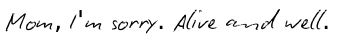
\includegraphics{Images/memo3.png}\\

The hasty scribble of just a few words had become a streak of light that
tore through the darkness, and became the voice that whispered life into
her ear.

Karan opened her store, and continued to bake bread. Until Shion came
home, she would grit her teeth and wait. She would keep waiting. Nezumi
had brought her the strength to do it. At times, she was still
overwhelmed with anxiety and the urge to scream, but Karan's daily life
was gradually regaining its stability. It was around this time that Safu
had appeared at her door.

Safu, like Shion, had also been acknowledged as highest-ranking in
intelligence. She was a girl whose large, black eyes stood out defined
on her face; and she had an honest gaze. Safu, with few words but a
strong will, had spoke of her love for Shion, and had proclaimed that
she was going to the West Block to see him.

"It doesn't matter to me. Even if I could never come back here again, I
wouldn't regret it. If Shion is in the West Block, that's where I'm
going."

"I want to see him. I want to see Shion."

"I... I love him. From the bottom of my heart, I've always, always,
loved only him."

The sixteen-year-old girl had formed these words, fighting back her
tears; and for their simplicity and awkwardness, they had touched
Karan's heart all the more. But moved as though she was, she could not
let Safu go to the West Block. As Shion's mother, and as grown adult,
she had to stop her.

Safu left her store, and Karan had followed shortly afterwards. What she
witnessed was the kidnapping of Safu by Security Bureau officials.

It had already been three days since then.

"Safu..." At her wit's end, Karan let another sigh escape her lips. She
had not the faintest idea what she was to do next. She had passed a memo
to the small messenger mouse. That was all she had done.

Would Nezumi save the girl as he did with Shion? If she was already
imprisoned in the Correctional Facility, it seemed almost impossible to
save her. If Shion found out, and set out to the Correctional Facility
to save Safu, perhaps this time he would really be killed. Maybe I've
done something rash― There was no way Nezumi would take such a risk to
save a complete stranger. Her feelings shredded into little ribbons, and
made her fingers tremble.

Karan had spent these past three days hardly sleeping or eating. She was
physically and mentally exhausted, and yet was unable to stay still, and
had come all the way here, close to where Safu used to live.

The luxury neighbourhood of Chronos.

Abundant greenery, and a tranquil environment. A fully-functioning
security system. Various facilities, for medical care, entertainment,
and shopping were provided in full, and residents could use them freely
with only their ID card. Even within the Holy City of No. 6, Chronos was
of a different class still, a residence beyond anyone's wildest dreams.

Although Karan had been a resident here only a few years ago, this time
she was prevented from even entering the streets. As soon as she had
stepped onto the cobblestone path that led into Chronos, the gates had
closed.

We are very sorry. Due to concerns for safety, the area past this point
is accessible to Chronos residents only. Thank you for your
understanding. Further, anyone who passes the gates without a Entrance
Permit for Special Residential Districts issued by the authorities is
subject to removal from the premises and punishable by municipal law
Article 203 Clause 42. I repeat ― Due to concerns for safety...

A gentle female voice flowed forth. The surveillance camera attached to
the chalk-white gates silently captured Karan as she stood with her feet
rooted to the ground. If she remained unmoving here, the soft voice
would turn into a shrill alarm, and Security Bureau officials would
burst onto the scene. Karan had no choice but to turn her back on the
gate, bite her lip, and go back the way she had come.

And now, in a corner of the Forest Park, she was sitting on a bench
under a large tree that had lost all of its leaves. She sat, staring
absently down at her hands.

"Shion... Safu..."

Why am I so powerless? I've been living for decades, I'm a parent, I'm
an adult, and I can't even help two young people who are in the middle
of a crisis. I've been alive for so long, and yet―

Karan lifted her face. An emotion quite different from dread or anxiety
flitted across a corner of her heart. In the years that No. 6 shaped
itself and began maturing as an independent city, Karan lived in its
interior as a resident.

Six cities were founded in this world, building upon the numerous
blunders that humankind had caused. It was a place free of war or
hunger, and people could live here in peace and freedom. Here, the
people could live from birth to death in safety, bliss, and tranquility.
That was how it was supposed to be. She had never thought deeply about
it. Everyone thought that as long as they stayed in No. 6, they would be
promised a fulfilling life.

They thought ― they had thought ― they had been taught into thinking.

She clenched her fingers, and bit her lip harder.

This is all a lie. Everything― it's all just an appearance.

She whispered without putting it into words. Though it was on the verge
of winter, she was starting to perspire.

They were divided into countless classes by their ID chips so that they
weren't even free to travel inside the city. Her son had been taken
forcibly into custody, and she was not permitted even to make a formal
objection. She couldn't even confirm the safety of another resident who
had been seized by the authorities. Where was freedom? Where was peace,
safety, and a life of fulfilment? It was nowhere.

If that's true, then what have we been doing all this time? Why have we
created a city like this? What have we done ― where have we gone wrong?

"Excuse me―"

Karan was jolted abruptly back to reality by a voice.

"I'm sorry. Did I surprise you?" An elderly lady wearing a small,
light-blue hat was smiling at her. It was a face she didn't know.

"Ah―oh no, it's nothing," Karan said hurriedly. "I'm sorry, I was just
lost a little in thought... is there something―?"

"Would you mind if I sat down beside you?"

"Not at all― please."

The woman, still smiling, lowered herself into her seat beside Karan.

"What splendid weather it is, don't you think? So nice."

"Yes, it is." The weather was the last thing on her mind. For the past
few days, she had felt nothing in the colour of the sky, the sound of
the wind, or the sight of the trees.

"You must have thought me a rather rude old crone for suddenly speaking
to you like that, I suppose?" the woman said mildly.

"No no, of course not. I was just a little surprised. I was thinking
about something, and I hadn't noticed that you were standing there."

The madam pushed her round spectacles up her nose, and her face turned
serious.

"You see, that's exactly why I decided to speak to you."

"I'm sorry?"

The woman was wearing a silver ring. Her fingers extended to clasp
around Karan's hand.~

"Please, I don't want you to be offended. I know very well that I'm
being meddlesome." She hesitated. "But you had such a forlorn look on
your face, I just couldn't go without doing something."

Oh, Karan said softly, her hands still clasped in the woman's.

"And that was why you took the time to speak to me?"

"Oh yes. There you were, on such a fine day, on such a splendid
afternoon, looking as troubled as ever. You were sitting alone, limp on
the bench, with your head bowed. There was no way I couldn't go without
saying something."

The elderly woman tightened her fingers around Karan's hands, and
wrapped them tenderly in her own hands.

"Why is a lady so young and beautiful as you, sitting with such a face?
Has something happened?"

The pair of eyes behind the spectacles were soothing and gentle. Above
their heads, the branches of a beech tree were swaying.

"Thank you for your concern. I've just been going through a bit of
trouble..."

"Yes, I understand," the woman said sympathetically. "There was a time
in my life, too, when I was burdened terribly with troubles." Her aged
but dignified countenance clouded slightly. Karan's heart leapt for an
instant.

Were there other people brooding like her? Were other people suffering
like her? Had other people realized the city's contradictions as well?

"It was devastating, even though it happened decades ago. ―I lost my son
to an illness."

"My, an illness," murmured Karan.

"Yes, and he was only three. When he died, I still remember crying
uncontrollably when I saw how small his coffin was. You would
understand, wouldn't you, the feelings of a mother who's lost her son?"

Karan tried to nod, and drew her chin back just in time. Shion was still
alive. I haven't lost my son yet.

"I can't quite say that I do understand―" she said slowly, "but you must
have suffered so."

"Indeed, I did. Words couldn't describe what I went through. Many times,
I thought how much better it would be if I were dead. But now, I'm glad
I'm alive. I couldn't be happier, living in such a brilliant city,
surrounded by my children and grandchildren."

The woman smiled, and cast her gaze around her.

"I would've wanted my son to experience growing up here. No― if medical
care at No. 6 had been what it is now, I'm sure he wouldn't have had to
die."

Karan softly drew her hand back. The elderly madam's gaze wandered into
the sky as she continued talking. Her lips were still turned up in a
vague smile.

"I really do think this place is a utopia. You know, I say this to my
grandchildren very often. I say, you must be grateful for being born
here. They just look puzzled, of course ― but that's when I tell them
about the West Block."

"The West Block?" Karan's heart quickened again, for an entirely
different reason this time.

"Yes, the West Block. Do you know what sort of place it is?"

Karan leaned forward. She wanted to know. The West Block was where Shion
was, and she wanted to know the details, what sort of place it was.

"I haven't the faintest idea. Please tell me."

The lady furrowed her brow, and shook her head.

"I don't know much about it, myself. But my nephew works at the Access
Control Office, and I hear stories from him sometimes. It's a horrible
place, I hear."

Karan restrained her impatient heart, and murmured in assent. She wanted
to encourage the madam to continue her story.

"The hygiene there is absolutely atrocious, and I hear the children have
to drink contaminated water."

"Contaminated..."

"Yes, isn't it just horrid? I feel such pity for them, my heart aches.
Compared to that, the children in this city couldn't be happier.
Wouldn't you agree?"

"What? I mean― yes, but..."

"That's why over there, they're plagued with contagious diseases all the
time, ones we could never imagine within No. 6. Crime is a daily
occurrence, and safety is almost nonexistent. The residents of that
Block are all uneducated, savage, and most will even kill a man without
batting an eye if it means money for them. Just recently, I heard a
group of violent men tried to force their way into the Control Office.
Of course, since their security system was perfect, they were arrested
before they even set foot inside. It's frightening, really."

The lady wrapped her arms around herself and shivered.

"My nephew told me the place is like a hell, the basest, worst possible
environment. It must be ever so different from here. We must rejoice
too, that we're residents of No. 6 ― not just our children. As for
myself, I'm not afraid to tell my grandchildren how fortunate they are
as No. 6 residents, compared to the West Block."

The West Block. The basest, worst possible environment.

Karan closed her eyes. Shion's handwriting floated up in her mind. It
was a mere scribble, and only one line long. It was a slightly slanted,
distinctive hand.

The letters were brimming with energy. It was writing that radiated
youthful vigour for life. He was alive in the West Block. Ever so
strongly, even now, he was continuing to live on.

"Is something the matter?"

She opened her eyes at the elderly lady's words.

"Are you feeling ill? Shall I contact the Health and Hygiene Bureau?"

Karan slowly shook her head.

"I don't think so."

"Pardon me?"

"I don't think the West Block is the basest, nor the worst."

"Why, what―"

"And I don't think―"

I don't think this city is a utopia, either.

Just as she was about to say those words, there was a sound, a flurry of
beating wings, and a black object came flying at her from above.

The elderly woman gave a small cry.

"Heavens, a crow!"

A crow with glossy black wings had alighted on the ground at Karan's
feet.~

"How disturbing," the woman said uneasily. "Were there ever any crows in
the Forest Park?" She furrowed her brow.

"This is a natural environment after all. There are crows, though
probably not many of them," Karan replied. The crow took flight again.
She thought it would fly away, but instead, it flapped its wings busily
and alighted again, onto a man's shoulder.~

It was Karan who gave a cry of surprise this time. She had not noticed
at all that there was somebody standing this close by. During her
conversation with the elderly woman, there had been other passerby: an
elderly man with his dog; a girl stooping to pick up a coloured leaf; a
group of what looked to be students ― but no one with a crow on their
shoulder. When had he gotten so close? How long had he been there? It
was a little unnerving.

The man was tall and wiry, and clad in a light-brown jacket, with
trousers of the same colour. He had a full head of hair, but with
streaks of grey that stood out. His moustache was also flecked with
grey. Apart from the fact that he had a crow perched on his shoulder, he
seemed like an ordinary middle-aged man. And he was a complete stranger.

But the man extended both his hands toward Karan with a smile on his
face. He even called her name as he spoke.

"Karan, I missed you."

"Huh?"

Before she could give a decent answer, the man grabbed Karan by the arm,
and drew her toward him. Karan's small stature nestled easily into the
man's long arms as they encircled her. He was holding her so tight, she
couldn't breathe.

"Forgive me," he pleaded. "It's all my fault. I'll never do anything
that'll make you feel bad again. I promise. You'll be the only one I
love for the rest of my life."

"Sorry, what―?" Karan stammered in alarm. "What are you doing?"

"I didn't realize how much I loved you until you were gone. Please, I'm
begging you. Say you'll start over with me again, Karan."

Why, he's gone mad.

Her first thought was that he was out of his mind. But if someone was
insane, they wouldn't be able to roam on city premises. Just as the
thought crossed her mind, she noticed the man's heartbeat. They were so
close to each other that she could feel his heart beating on her own
chest. It was beating with a steady rhythm. The man was neither insane,
nor nervous with excitement. He was very much coolly and calmly rattling
off these clichéd lines.

"I don't believe this. I've had enough!" Karan thrust her arms in front
of her, and pushed the man away. "I've had enough of your sweet-talking.
I'm leaving you. I never want to see you again."

"Karan, I love you. I'm really, seriously, in love with you." The crow
on the man's shoulder cawed shrilly, as if to mock them. The man cleared
his throat awkwardly, and bowed his head to the elderly lady, who was
staring at them with her mouth gaping open.

"I'm very sorry for having to show you such an ugly scene."

"Oh― ah, you don't need to―" the woman said falteringly. "So, er, you
two are―?"

"We're lovers," the man answered. "I was a fool, and I caused her a lot
of pain. I just wanted to apologize to her, and start over again."

"I see. Well, that's..."

"We've got some important things to discuss, so if you'll excuse us―"

The man grabbed Karan's arm, and she was half-dragged away from the
scene. The crow cawed loudly again. They took a back route behind the
Park Office ― Shion's former workplace ― and exited through the back of
the park, the man uttering not a single word the whole way. Karan also
remained silent as she was pulled along by the arm.

There was a white car parked at the curb. It was a rather old model,
seldom seen on city streets anymore. The man opened the door, and spoke
quite without any hesitation.

"Get in."

"No, thank you."

"Get in," the man repeated. "I have something I want to talk to you
about." With a great swoosh of its wings, the crow swooped noisily from
the man's shoulder to the back seat of the car. Then, it looked at Karan
and jerked its head, as if to invite her to follow.

"He looks like a smart bird," Karan observed.

"He's a little too smart for his own good." The man's long-suffering
tone was telling of how much trouble the bird must have caused him. The
crow opened its beak widely and made a cackling sound. It sounded like
it was laughing. Karan, found herself laughing a little, too. Only after
she finished laughing did she realize how she had gone these past few
days without laughing, or even smiling at all.

Karan continued holding the crow's gaze as she slid into the passenger
seat. The electric-gasoline hybrid car glided forward soundlessly. When
they merged onto the highway, the man pressed the switch on auto-drive
and took his hands off the steering wheel.

"Did you know? A new bylaw is being put into place, and we won't be able
to use gasoline starting as early as next year. Which means I won't be
able to drive this car anymore either."

"I've heard that fossil fuels have nearly been depleted, except for
coal," said Karan. "I guess we wouldn't have any other choice but to
switch to another energy source."

"Who did you hear that from?"

"Who―? Well, it's been announced in the city's energy policy―"

"Exactly. An announcement by the authorities. The mayor's speech on his
administrative policy, word-for-word." The man twitched his moustache in
a cynical smile. "No one questions it. Everyone accepts what the city
announces as it is, and agrees to it without a thought. God, everyone in
this damn city is so obedient and naive. Doubting their superiors is the
last thing on their minds. They probably can't even imagine doing that,
or want to. Having suspicions takes energy. It's easier just to sit back
and say, yes yes, I agree, to everything."

Karan threw a sidelong glance at the man's face.

Then are you saying that you have suspicions? Instead of nodding
obediently, are you saying you're stopping to question it?

She resisted the urge to ask him. It wasn't wise to say such reckless
things to someone she barely knew. She had to be cautious, like a
cowering herbivore.

Karan drew herself up, and tried to change the direction of the
conversation.

"May I ask you a question?"

"Fire away."

"Who are you, and how do you know my name? What made you go so far as to
stage that half-baked act to pull me out here?"

"Half-baked is a little harsh, no?" said the man wryly. "I thought I
pulled it off quite well. You played along nicely, too. That's Best
Actress Award material."

"Why, thank you," Karan said pleasantly. "The role of romantic heroine
isn't one I get to play often at this age."

"Well, I don't see why not. You're young and beautiful enough, quite,
quite. You could play any heroine you wanted, Karan."

"Where did you learn my name?"

"From my niece."

"Niece?"

"Says she's a fan of yours," said the man. "Or I should probably say, a
fan of your muffins."

A small, round face floated up in Karan's mind ― the girl who always
came to the store with coins clenched in her fist.

"Ma'am, you won't close this bakery, would you?" ― The girl who had
shown sincere concern for Karan. She, along with the words and gazes of
encouragement from others, had supported her in her dark days after
Shion had been taken into custody by the Security Bureau.

"Lili."

"That's the one," the man affirmed. "Lovable Lili. She's my younger
sister's daughter. Says she likes your cheese muffins a hundred times
more than ol' Uncle here. She told me last time I saw her."

"Oh, dear."

"I was ticked off, so I was going to put in my own two-cents about these
muffins of yours, and took a bite out of one to taste..." The man's
mouth made a chewing motion. He poked the tip of his tongue out, and
licked his lips.

"They were good, weren't they?"

"They were. I hate to admit it, but they were delicious. Guess it can't
be helped that Lili would like them more than some old uncle who only
pops by once in a while."

"Well," said Karan, "at least now I know that you're Lili's uncle, and
that you learned my name from that adorable niece of yours."

"Thanks for understanding. Did you think I was someone suspicious, by
any chance?"

"I still do. What was that act back there? Did you want to pull me away
from that respectable madam that badly?"

"You bet. She was dangerous."

"Dangerous?"

The car turned slowly. It was going into Lost Town. It seemed safe to
believe that this man intended to take her home.

The old car went back along the same path she had taken this morning,
deep in thought. She had taken a day off from the bakery today. Was Lili
disappointed?

"You were a hair away from voicing your dissatisfaction toward the city.
Am I right?"

I don't think this city is a utopia.

Indeed, she had been about to voice those words. But she had been
interrupted at that very moment by the sound of the crow's beating
wings.

"That was dangerous?"

"There's a possibility it might've been. What would you have done if
that lady decided you were trouble?"

"Trouble? What do you mean?"

"What I'm saying is, she would've gone to the authorities and told them
that the women sitting on the park bench has a dissatisfaction with the
city."

"You mean she would secretly turn me in?"

"Finding it hard to believe?"

"Of course," Karan blurted. "That's nonsense. That madam was concerned
about me. She spoke to me out of kindness."

"Exactly, because you looked so depressed. In this utopia, in No. 6,
everyone has to be happy. Even seriously ill or injured people have
almost all of their pain removed by leading-edge medical technology.
People who are troubled, or who contemplate, or who lose themselves in
thought ― those kinds of people don't exist. They aren't allowed to
exist."

"That's not―" Karan protested. "I mean, there are always people on the
bench who seem to be lost in thought."

The man shook his head, and tapped a corner of the small monitor on the
dashboard that was displaying road information. Small digits expressing
the time popped up on the screen.

"Do you remember how long you were sitting on that bench for?"

Karan gazed at the numbers, and shook her head. She had forgotten
completely about the time. She had sat on that bench, contemplating,
wrestling with her thoughts, and unable to find an answer. She had lost
the will to stand up and keep walking.

"Your time limit is thirty minutes," the man muttered.

"Huh?"

"Citizens are allowed to space out for thirty minutes, at the most. If
they're thinking deeply or losing themselves in thought for longer than
that, the flags come up and someone'll jump in to check."

"So you're saying ― that madam approached me to investigate, because I
was brooding for such a long time?"

"I couldn't say," the man answered. "All I know is that there was a
possibility. Maybe she was just a little old woman who thought she was
being kind and generous ― the kind that won't mind doing something nice,
as long as it's not too much trouble for them."

"What a horrible way to put it."

"It's the truth. This city is teeming with those kind of self-proclaimed
good Samaritans. There are so many of them, it gets pretty hard to
distinguish the ones that are actually good. Still, if that madam was
one of those, it wouldn't be a problem. But what if she was a snitch?
That would've been a close call for you, wouldn't it?"

Karan didn't answer him. She didn't want to be suspicious of the elderly
madam. She wanted to believe that the woman had been a kind soul who had
spoken to her, a stranger, out of genuine concern.

She had had such gentle eyes, smiling behind her spectacles―

Karan drew a sharp breath.

"Those glasses..."

"You've finally noticed? They were a little big and clunky for a
sophisticated madam like her, don't you think? Maybe they were built in
with a microphone and recording device."

Karan closed her eyes, and let out a long breath.

Thirty minutes was her time limit. She was not allowed any more.

To contemplate deeply; to wrestle with one's thoughts; to immerse
oneself in the realm of one's mind; and from there, to find one's own
answer ― it was all prohibited.

The same question welled up inside her breast again.

What have we been doing all this time? Why have we created a city like
this? Where have we gone wrong?

She swallowed her sigh. She felt exhausted, and felt as if the mental
will to retaliate, and the strength to become angry, had all withered
within her.

"I've probably been tracked by the authorities all this time," she said
quietly. "They must have been keeping me under surveillance, and not
only because I was lost in thought. I am the mother of a convicted
murderer, after all."

"There'll be none of that," the man said sharply. "No putting yourself
down." His tone was that of a father scolding his daughter. "Do you
really think your son is a criminal, like the authorities have told
you?"

Karan lifted her gaze off the floor, and shook her head. She had not
believed for an instant that her son had murdered someone.

"This is also something I heard from Lili," continued the man. "She says
your son ― name's Shion, right? ― says he's really nice. When she'd
break her toys, he'd always fix them for her. Says she likes him a lot
more than Uncle here, though not as much as your muffins. She was
wondering if he had a girlfriend."

"Was she? Oh, dear," Karan said, with a hint of a smile in her voice.

"Cheeky, huh? Acting older than her age. But for all it's worth, she
can't seem to realize how attractive her own uncle can be. Don't know
how my sister raised her, for her to turn out like that."

"And if I ask Lili, would I be able to find out what name this
attractive uncle of hers goes by, and what he does?"

The man laughed at Karan's words, and tapped the panel lightly again.

"God knows what might happen if you asked Lili. She'd probably tell you
that Uncle Yoming is a weird man who wanders by the house once in a
while, eats 'til he's full, and scoots out of the place."

"Yoming. That's your name."

"Yeah. And this is my job."

The panel filled with images of bread, cakes and other light fare,
followed by caloric content and nutritional information, price, and name
of the stores that served them.

"I run an electronic newsfeed for all sorts of entertainment in the
areas, all of them except Chronos. Which isn't much, I mean, apart from
dining and seasonal events, which is mostly what I do. Since the city
oversees all the plays, concerts and print publishing, there's not much
we can write about other than food and drink. The Food Bureau's out of
the question, no way I could get inside that place ― so it's just stuff
like where to eat good cakes, or good places to have lunch, or things
like that. I do the best I can. It's actually quite popular. I mean,
after all, in Lost Town, there's not much to do for fun other than eat
or drink, so everyone's eager for information."

"Then by any chance, are you―"

"Right on," the man said energetically. "I want to run a feature on your
bakery's breads and cakes, with a spotlight on the muffins. Will you let
me interview you?"

"Are you sure you want to write about my shop?" Karan said worriedly.
"Won't the authorities turn their eye on you too?"

"I don't care if the authorities turn their eye on me, or want to trip
me up, what-have-you. I can't let those delicious muffins go without any
publicity." He paused. "Though Lili probably wouldn't be too happy if a
crowd of customers came and cleaned out your muffins. Uncle, you never
do anything right, she'd probably say."

"Never," smiled Karan. "―But my bakery's been on the news before, with
my son's incident, and all. People from Lost Town might still come ― but
what about people from other areas?"

Yoming shrugged his shoulders, and erased the image on the touch-panel
screen.

"Karan, the people of this city aren't very good at remembering things."
His voice was hoarse, and hard to catch.

"They forget everything at the blink of an eye. No matter how serious an
incident. Gone. What's more, they don't even see the possibility that
there might be something underneath the surface. Remembering, doubting,
contemplating. It's hard for them to do. But they don't even have to do
it ― the day still goes on, and peacefully, too. It's a terrifying
place, this."

Yoming's words sounded so much like an open criticism of the present
condition that Karan found herself straightening in her seat. If this
conversation reached outside ears, that would be more terrifying than
anything. As if perceiving Karan's agitation, Yoming relaxed his face in
a smile and waved his hand nonchalantly.

"Don't worry. This car is equipped with an anti-tapping device. But who
knows, maybe all the new cars rolling out next year will have tapping
devices built right into them."

"Yoming, why are you so critical of the city? How can you be so certain
that this is a frightening place?"

After a brief silence, Yoming tapped the touch-screen three times.

The image of a young, delicate-faced woman appeared. A baby was sleeping
in her arms, bundled in a white blanket. The woman's smile was filled
with the bliss of motherhood. Her chestnut hair, cropped in a short bob,
framed her alert and energetic face, and her gentle smile was memorable.

"My wife. That's our son in her arms. This picture is from a long time
ago."

"Did something happen to your―?"

"Same as with your son, she left the house one day and never came back.
The only thing that's different from your case is that she disappeared
along with our son, and that she was filed away as a missing person."

Karan's breath caught in her throat. Yoming's calm and levelled way of
speaking made the fact even more shocking.

It's the same as Shion― there's someone who's been through the same
thing―

"She was a school teacher," Yoming said quietly. "She taught art and
music to kids like Lili. Said no other job could suit her better. She
always told the kids to cherish what they felt in their hearts. Whether
it be for drawing a picture, or writing a song, she said the most
important thing was to look straight at your feeling and emotions, and
express them truthfully."

"That's beautiful," Karan breathed. "I don't think I've heard such
touching words in a long time."

"Yeah. She was an admirable woman, touched a lot of people. She had firm
beliefs, and taught her children based on those. But she started getting
more and more stern warnings and directions from the Education Bureau...
they told her to teach the kids strictly by the book. The book that
they'd published, of course. Naturally, she resisted― and she got fired
from her workplace. She got her license revoked too, because they deemed
her as unfit for teaching. I think during that time, there were quite a
few teachers like her who were removed from their jobs. You didn't know,
did you?"

"I had no idea― I can't even remember..."

"No need to be ashamed. It's natural you shouldn't know," Yoming said
grimly. "It didn't make the news. The authorities were already starting
to manipulate information by that time. There you had the seeds of a
system that would eventually prevent anything inconvenient from being
publicized as tangible information."

The car was already entering Lost Town. This district was always the
least-maintained and the last to be updated in its facilities, and was
an area of haphazard mish-mash. Amidst its restless buzz, Karan found
herself sighing a breath of relief.

"She was planning to build a school for children, with other exiled
teachers ― she was trying to teach in a place where the authorities
would have less influence. She'd left for a meeting to discuss plans for
the school that day ― and she never came back."

Yoming clenched his fist, and pounded the steering wheel. The crow cried
plaintively in the back seat.

"I'll never forget," he said through clenched teeth. "No matter what
happens, I'll never forget. I'll keep it alive in my memory. It was
cloudy that morning, and it looked like it would rain any minute. I'd
gone to the dentist because my toothache was getting unbearable. I was
off work that day, so I should have been the one babysitting our son at
home. But she took him with her so I wouldn't have to. She put him on a
stroller with a blue hood, and she was wearing a beige jacket. There
were small embroidered flowers on the chest. We promised that if my
toothache settled down in the afternoon, and it didn't rain, we'd go out
to the Forest Park to take a walk. At the door, we kissed and said
goodbye. I kissed my son on the cheek, too. He laughed, and kicked his
feet. He was wearing tiny little white socks. There were flowery
patterns sewn on them too. They were purple violets. I still remember. I
still haven't forgotten a single thing. I could never forget."

"Yoming..."

The car stopped.

You have arrived at your destination, announced the car navigator. They
were in front of Karan's bakery.

"I'm sorry, I got a little worked up," Yoming said. "Rude of me, since
we've only just met."

"No―" Karan said softly. "Thank you for bringing me home."

She paused uncertainly. She questioned herself whether it would be
alright to tell him about Safu. She was unable to decide whether she
could completely trust the man in front of her.

"Ma'am!"

Someone rammed full-speed into Karan's waist as she got out of the car.

"My, Lili."

"Ma'am, why did you take a day off today? Are you sick?"

Yoming called over from inside the car.

"Lili, she's fine. Madam here just had some errands to run. She'll bake
muffins for you tomorrow, I'm sure."

Lili blinked, and her mouth gaped open.

"Hey, is that you, Uncle Yoming? Did you come to eat dinner again? Why
do you always come when we're having chicken and mushrooms?"

"See, this is what I get. Horrible, isn't it?" Yoming smiled wryly, and
leaned forward to peer into Karan's face. "If you can, open your bakery
again tomorrow. And keep on at it. You've got a job to do, Karan."

"Of course."

"Never despair. You can't give up, no matter what. It's only when you
despair and decide that there's nothing you can do, that you really
lose. It might seem easier to just give up―"

Karan placed a hand on top of Lili's head, and shook her head firmly.

"No, I won't give up. I have my responsibilities."

"Responsibilities?"

"Yes. I'm a grown adult, and I've been living alongside this city for a
long time. I've done my best to live respectably, but if the result of
that is what this city has become ― then we've made a huge mistake
somewhere along the way. I'm not sure where we've made it ― but I know
I've got to take responsibility for it. We can't let children like Lili
suffer because of a crime that's not their own, right?"

"Shh―!" Yoming lifted a warning finger. A young woman on a bicycle sped
past the car. "I understand how you feel, but don't say those kind of
things out loud here. You don't know who might be listening."

Lili giggled, and pulled at Karan's skirt.

"Uncle Yo's always being cautious. He's a scaredy-cat, even though he's
a grown-up."

"When you grow up, Lili, you'll start to understand what the really
scary things are."

"Well, I think Mommy is the scariest when she's angry," Lili said
matter-of-factly. "She's really scary, you know. Daddy says he's scared
of Mommy the most, too."

"Ah, that's right, of course," Yoming replied gravely. "I agree, your
Mommy can be very scary."

Karan burst out laughing. Lili's mother would often scold her children
in a booming voice that was hard to imagine coming from her slender
frame.

"Lili, Yoming, and Mr. Crow, too ― if you have time to spare, how would
you like to stop by for a bit? I wouldn't be able to serve you muffins,
but I could whip up some pancakes."

"Really? Yay!" Lili clasped Karan's hand tightly. Her hands were soft.
Karan's heart swelled with an outpouring of love.

I can't let this little girl go through what Shion and Safu did. And I
must save those two, somehow. Yes ― we have a responsibility to fulfill.

Her eyes met with Yoming's. They stared back at her, the colour of
crow's feathers. Karan nodded, and unlocked the door.

"Lili, come in. You too, Yoming. I still have things to speak to you
about."

Just then, a small black spot flitted across her vision. She heard the
buzz of wings.

"What's wrong?" Yoming followed Karan's gaze and glanced around as he
got out of the car.

"There was an insect ― I thought I saw a bee flying around."

"Bee? It might be warm still, but I don't think they should be active
anymore."

"I guess you're right."

It was winter. There was no way bees would be flying around. Even if
there were, it was probably a single insect that had wandered out into
the air, drawn by the sunlight and warmth. But she could not shake the
foreboding feeling in her heart.

"Ma'am?"

Lili stared up at her from below as she stood still in the doorway.

"Oh, sorry about that. Come on in."

My nerves are just on-edge. I must be tired. Karan reassured herself,
and opened the door. She stepped inside, and shook her head violently,
as if brushing away the buzzing sound that had lodged itself in her
ears.

\hypertarget{index_split_034.htmlux5cux23calibre_pb_66}{}

\protect\hypertarget{index_split_065.html}{}{}

\hypertarget{index_split_065.htmlux5cux23calibre_pb_0}{}

\hypertarget{index_split_065.htmlux5cux23calibre_toc_4}{%
\subsection{CHAPTER 3}\label{index_split_065.htmlux5cux23calibre_toc_4}}

\subsubsection{Land's End}

\emph{Humans were born from the eye of Ra. Ra was the creator of heaven,
earth, and all things. Since he was the Sun, and also the ruler of the
gods, it was decided that he would become the first King on earth.}

\emph{-Egyptian myth 'The Beginning of Heaven and Earth'~}

It was blurry. Everything was veiled in a haze, and vague.

But I have to wake up...

Safu struggled to open her eyes. She bit her lip as hard as she could.
There was a slight pain. She could feel her sensations returning.

Safu realized that she was bound to a stretcher. A white door opened,
and she was carted inside. In her blurry vision, she could not make out
what was there. She felt her body gliding sideways.

"Ah, are we awake?" It was a man's voice. "No need to be, though. Let's
give you an anaesthetic, shall we? Then you can sleep again in peace."

"Where... am I...?"

"Care to take a guess?"

What's wrong with me? What happened―? I visited Shion's house, and then―

There was a man in a Security Bureau uniform.

'Are you Safu-san?'

The shock in her neck. The numbness that had spread through her body.

Safu almost shrieked in terror. Her lips parted, but no sound came out.
Her voice was stuck at the back of her throat.

"Correc...tional... Facility..."

High-pitched laughter rang out. The man was laughing.

"Do you fancy the Correctional Facility? It seems you've taken a liking
to it. I know, once this surgery is over, you can live in your own
special suite until you die. I'll have it all arranged."

Surgery?

"Surg..."

"Yes. You're lying on a surgical table." The man's voice was still
filled with mirth. A white glare filled her vision. Safu took it to be
the light of a surgical lamp. She was pierced with horror ― stronger
than the horror that had seized her when she had been apprehended by the
Security Bureau.

A tear spilled from her eye.

"There's nothing to cry about. There will be no pain, or discomfort.
Good night, now."

Shion. Shion. Shion.

This name will protect me from all evil things.

He'll save me. He'll rescue me, and get me out of here ― Shion.

"Shion."

His name was called. Shion stopped his feet. His guard, a large dog,
gave a low growl.

"Rikiga-san."

Rikiga was exiting a shabby restaurant through its rickety glass door.
Shabby as it was, it was one of the more decent establishments in the
West Block's bazaar. Most establishments of these sort were clusters of
barrels and crates placed outside to sit on, and the dishes were all of
an unidentifiable origin. The stench of strong spirits and some
mysterious stew wafted out from these stands out into the street, and
Shion often found himself pinching his nose. But even so, starving
children and old beggars milled about the shops, some wandering in hopes
of receiving food, others staring fixedly at the adults bringing their
food to their mouths. A shop owner raised his voice angrily, splashing
water outside his storefront, and chased the people away as if they were
stray dogs or cats.

And in front of these starving people, those who had been able to get
their hands on the day's sustenance sank their teeth into their food,
dripped grease over their mouths, and licked their fingers.

To have money, and to have power.

To have food meant to fulfil these conditions.

Shion had learned this from these few days here. But he still could not
get used to it. He couldn't bear to look at the scene before him. He
couldn't help but avert his gaze, and look at the ground.

"If it makes you feel better, then give them a handout. But only if you
can fill the belly of every single person there," Nezumi had said. For
Shion at the present, it was an impossible task.

"What can you do with your half-hearted sympathy? You might be able to
save a handful of kids from starvation, for a short time. But that just
means you're creating two new types of people― those who are starving,
and those who aren't. Let me tell you something interesting, Shion. It's
more excruciating for people who've filled their belly once to starve,
than for people who have never been full at all. Nothing is more harsh
than starvation after satiation. These kids here have never eaten until
they're full. They don't know what it's like to be satisfied. That's why
they can put up with it. Understand? There's nothing you can do here,
absolutely nothing."

Nezumi had spat those words, and strode out of the room. But before
that, he had stopped abruptly before the door, and turned around. A
brown dog was sprawled off to the side.

"So Inukashi's lent this dog to you as your bodyguard, huh? And I hear
your wages were a little more flush than usual. Looks like you've become
his favourite."

"He says he'll let me continue working for him. He asked me to clean the
guest rooms and take care of the dogs."

"And you took the job?"

"Of course," Shion replied enthusiastically. "I was so happy, I thanked
him over and over again."

Nezumi sneered.

"Will you look at that. Mr. No. 6 Elite is rejoicing over a
housecleaning and dogkeeping job. It should be interesting to see how
much lower you're going to stoop."

"I don't think I'm stooping," Shion said promptly. "You'd agree,
wouldn't you? You don't think this is stooping at all."

Nezumi's shapely face contorted slightly. He hunched his shoulders.

"Oh yeah, Shion. You got paid by Inukashi today, didn't you? Go out and
buy some dried meat and bread."

"At the market?"

"You don't know any other place to buy food, do you?" Nezumi said
sarcastically.

"Well―yeah, but..."

"Dried meat and bread. Inspect it carefully when they give it to you.
Space out like you usually do, and you'll be stuck with a mouldy brick
of a loaf. And haggle. Haggle like no tomorrow. I'm off."

The door closed, and his footsteps faded into the distance.

He would have to buy dried meat and bread in front of those children.

Nezumi had told him to.

Dried meat, and bread.

Shion's stomach growled insistently. His mouth watered. He had had only
the slice of bread and fruits that Inukashi had given him at noon. He
was terribly hungry. He had not eaten any meat, nor soft bread, for
days.

His stomach growled, his mouth watered.

He wanted to eat. He wanted to sate his empty stomach.

Shion sighed, and pulled his hat further down over his head.

What can you do with your half-hearted sympathy?

He recalled Nezumi's words again and again.

You're right. I can't do anything. I'm just pretending to pity those
kids to boost my self-respect. The truth is that I'm about to buy meat
and bread, right in front of those children, to satisfy my own hunger.
That's my true form ― that's the kind of person I am. Nezumi, is that
what you meant?

There were a few coins in his pocket. It was his day's payment that he
had received from Inukashi.

"Part of that is a thank-you for treating my brother. I can't always pay
you this much." Inukashi had said this rather curtly, but Shion was
grateful for his kindness. It may have been quite a large amount for a
day's worth of work. But even so, it was enough to cover only a few
strips of dried meat and two or three loaves of mouldy bread. There was
almost no food left in their room, otherwise buried in books. He
wouldn't be able to live off Nezumi's goodwill forever. He had to secure
a means of providing for himself, however little it was.

Shion pushed the door open, and stepped outside. The dog slowly got to
its feet, and trailed after him. When Shion set foot into the market
street, it drew up to Shion's side and kept pace with him closely. He
was trained well. It was apparent that Inukashi had quite a hand with
his dogs. Shion smiled sheepishly as he caught himself, yet again, being
surprised or impressed like with so many other things since coming to
the West Block.

It was already dusk. Darkness was setting in, and the cooing and
bellowing of voices echoed even more loudly in the air. Under ripped
tents, and in front of barracks, people sold and bought things, ate, and
drank. As soon as the warmth of the afternoon slipped beneath the
horizon, the ground beneath them grew colder by the minute. Business was
probably booming at Inukashi's hotel. For those who had nowhere warm to
sleep, it was going to be an unpleasant night. Bare-breasted women
called out from the darkness of the alleyways, and old women clad in
rags huddled on the ground in the same darkness. Children trotted about,
nimbly threading through the crowd, and being yelled at occasionally.
And still people bought and sold, ate, and drank.

Don't know what waits for me tomorrow. But at least I've lived through
today.

So I'll eat. So I'll drink. Here, it's everything we've got.

All the things I've said, can't enjoy 'em once I'm dead

So I'm alive an' enjoyin' 'em today.

That's everything. Here, it's everything. My everything.

Someone was singing off-key. Shion paused, and tilted an ear to the
voice. He hugged the parcel of dried meat and bread that he had just
bought close to his chest. This clamour that seemed to rush at him and
overwhelm him ― this clamour, this jumble of noises that seemed to burst
out of the ground itself ―

It was all connected to those who had a strong attachment to life, and
the energy that they radiated. Here, everyone clung fast to life. They
greedily latched onto survival. Because nothing insured a tomorrow for
them, these people lived with even more desperation. This energy, this
clamour. It was something that didn't exist, wasn't allowed to exist, in
No. 6.

What feelings did Nezumi have as he walked through these streets?

"Brother."

A feeble voice called out to him. He turned to see a thin child robed in
faded cloth. He had long, matted hair, and a dirty face. Shion couldn't
tell whether it was a boy or a girl.

"Spare some bread for me," the child pleaded weakly, in a voice that was
barely a whisper. "I haven't eaten for three days. Please, just a
morsel."

The child's countenance reminded him of a little girl he got along with
back in Lost Town. Her name was Lili.

"A morsel..."

A pair of tiny hands stretched toward him. Almost without a thought,
Shion was putting his hand into his parcel. As soon as he pulled out a
round roll, an impact slammed into his back. He had been shoved. He
staggered. As Shion lost his balance, a pair of small hands snatched the
parcel from Shion's arms. At the same time, he was shoved violently in
the back once more, and he fell to his knees.

"Run!"

The child shouted energetically, almost unrecognizable from the whisper
moments before. Several children yelled after him as they stormed past
Shion. The dog leapt forward swiftly and silently. He attacked the child
who had stolen the parcel. Screams rose from the group.

Still hugging the package of dried meat and bread in both hands, the
child crumpled to the ground. A few strips of meat and a piece of bread
fell out and scattered on the ground. The dog pinned the child down with
its legs, and bared its teeth.

"Stop it! Heel!" Shion had shouted without thinking. The dog obeyed,
closed its mouth, and looked up at Shion reproachfully. The child didn't
miss his chance. He sprang up, and broke into a sprint with the package
in his arms. He moved with the swiftness and agility of a wild animal.
In moments, his small back had disappeared into the throng. The other
children had also melted into the crowd, out of sight.

"Amazing..."

Shion couldn't help but murmur at their cunning ways. Admittedly, he was
impressed. He soon realized that this was no time to be impressed, and
stooped to gather what was left of his meat and bread. What would Nezumi
say, after seeing it reduced to almost one-third of its original amount?
Would he say nothing, and shrug his shoulders? Would he sneer?

Shion shrugged off his coat and wrapped the bread and meat with it. He
would share this with Nezumi for dinner tonight. Those children would
probably do the same. They would share it amongst themselves, and each
have a tiny morsel of food for dinner. Naive, and meaningless sympathy.
He knew Nezumi would criticize him scathingly, but Shion was still a
little relieved.

At least tonight, those children would have food. Right now, he had no
power to free them from starvation. He couldn't do anything. But if his
meat and bread would stave off their empty stomachs even for a short
time― wasn't that at least a little meaningful? It was acceptable enough
to give up because he was powerless to do anything. It was acceptable,
but it was arrogant. Wouldn't you think so, Nezumi?

"Oy, you there, fella."

From a stall selling roasted kebabs, the female shopkeeper called over
to him in her raspy voice. "Will ya stop standin' in front o' my store
all dazed-like? Being a nuisance, you is. Disruptin' business!"

"Oh, I'm sorry," Shion bowed his head hastily in apology, but the shop
mistress was already busy dealing with other customers to notice him.
Here, no one looked out for other strangers. They simply weren't
interested. Whether there be robbery on the street, or a beggar dying,
or a fight breaking out, no one cared. It all blended into the scenery
of daily occurrences.

"Well, let's go home, then," Shion called over to the dog, and noticed
its jaws snapping as it was chewing something.

"Hey, wait a minute, don't tell me you're―"

The dog gulped the meat in its mouth, and looked up at him with a flash
of a grin.

"When did you manage to pick that meat up? A lot quicker than me, huh."

The dog lolled its pink tongue, licked its chops, and began trotting
briskly ahead of him. Shion was amused, though he wasn't sure why.

He had been following the dog for some time when he was stopped by
Rikiga. Outwardly, Rikiga's job was publishing lewd adult magazines. But
behind the scenes, he acted as a middleman for prostitutes, and that was
his livelihood. Among his patrons there were said to be higher officials
of No. 6 as well. In the words of Nezumi, it was from these kinds of
people that Rikiga cunningly weaselled great amounts money.

But he was also the man that Shion's mother Karan told him to go to for
help. According to Rikiga, a long time ago before No. 6 and the West
Block was been divided with a wall of special alloy, he had met and
fallen in love with Karan. But it was only he who had fallen in love,
and Karan had merely shown agreement toward the articles that Rikiga had
written as a journalist at that time.

"He's the prime example of a corrupted man." These were also Nezumi's
words, but Shion found he liked the somewhat aloof and fearless aura of
the man who had once loved his mother. This man wasn't completely
corrupted. He still had journalism in his bones. That was what Shion
felt.

Rikiga's face was beet-red from drunkenness, and even his eyes were
bloodshot. It looked like he had been drinking quite a bit.

"Rikiga-san, it's bad for your health if you don't lay off the alcohol a
little."

"You're so kind, Shion. I feel like Karan's the one reprimanding me. She
was just saying to me the other day, 'Please, Rikiga, mind your
health.'"

"The other day? My mother?"

"In my dream. Ever since seeing you, Karan's started appearing in my
dreams. And every single time I see her, she scolds me. Don't drink,
don't be reckless, don't lose sight of what your job should really be―"

A flush that was not from alcohol rose in Rikiga's cheeks. He turned his
face away as if to avoid Shion's gaze.

"Well, a dream's just a dream. Karan's moved on, gotten herself an
admirable son like you. I'm sure she's changed from when she was younger
― in appearance, and heart too."

"She's aged," Shion conceded. "And she's gotten a little plump. ―But if
she were to see you again, Rikiga-san, I'm sure she'd say the same thing
she said to you in your dream. That's the kind of person she is."

Rikiga opened his mouth to say something, and then pursed his lips.

"All that about Karan― it's― it's alright. To tell you the truth, it's a
bit painful remembering..." he trailed off before abruptly changing the
subject. "So are you alone today?"

"I'm with the dog."

"The one that's glaring at me suspiciously right now? You wouldn't wanna
bite me, mutt. Just so you know, my meat is soaked in booze, and it's
running in my veins. Sink your teeth into this, and you'll go belly-up
from alcohol poisoning."

The dog glanced up at the drunken man, twitched its nose disdainfully,
and scowled. Shion looked down and chuckled to himself.

"What's his problem?" Rikiga grumbled at the dog. "So, no one else with
you today apart from the dog?"

"Are you talking about Nezumi?"

"Yeah. That sarcastic smart-aleck of an actor. Geez, I don't think I've
met anyone as foul-mouthed as he is."

"But you were his fan, right?"

"I just didn't know his true identity, that's all. I mean, Eve is quite
enthralling onstage. I never would have guessed that he'd be such an
impolite asshole. The kid goes around saying whatever he wants, whenever
he wants. Hard to imagine how a beautiful face like that can be so brash
and brutal. Unbelievable, I tell ya."

"Nezumi only speaks the truth."

No matter how harsh or ruthless his words were, they never carried any
lies. That was why they became blades and spears that pierced Shion's
chest, and left a pain that he could not forget. It was a pain that he
would never have known if he had not met Nezumi. Every time the
countless pangs stirred restlessly deep in his chest, Shion felt
something in himself changing little by little. A part crumbled away,
while another part rebuilt itself; and yet another part would be born
anew. Each word from Nezumi, and the pain that accompanied it led Shion
to change, and kept urging him forward. Shion could vividly feel himself
being changed and shaped by the force of another.

"You know, Shion. If it gets too unbearable, you can stay over with me,"
Rikiga said as they walked side-by-side. His breath hit Shion's cheek,
and reeked of alcohol.

"Unbearable? What do you mean?"

"No, I understand," Rikiga said abruptly. "You don't have to hide it. I
can't imagine how it wouldn't be unbearable living with Eve. I'm
guessing your living conditions are less-than-standard. Are you getting
enough to eat? Now, I think this highly unlikely, but if in some nasty
turn of events, you get influenced by Eve and your personality gets as
twisted as his― hm," he grunted to himself. "Indeed. There's no way I
can let that happen to Karan's son. Come live at my place. I'll give you
enough to eat, and give you a warm bed to sleep in."

"No, that's alright. I'm fine."

"But Karan sent word to come to me for help, right?"

"Yes, but I don't want to be a burden on you, Rikiga-san," Shion
insisted. "I'm fine. I've managed until now, and I'll keep managing. And
I actually enjoy being around Nezumi."

"There's no way you'd enjoy being around an ass like him. You don't have
to put on a brave face. You're having a hard time, aren't you? Look,
you're not even wearing a sweater. You poor kid."

"Oh, no, I'm just using my sweater to wrap my meat and bread―"

But Rikiga wasn't listening to Shion's answer. He was glancing at his
surroundings, and nodding fervently to himself.

"I know a good store. Let's go there." He yanked Shion by the arm, and
walked into a shop that was lined with an enormous quantity of clothes.
It looked like a used-clothing shop, and there were garments even
hanging from the ceiling. The clothes ranged from well-worn to almost
new.

"G'day." A woman almost as large as the shopkeeper from the kebab stand
materialized out of the shadows of a mountain of clothes. As soon as she
noticed that Rikiga was her customer, she pasted a bright business smile
onto her face.

"Whah, Mr. Rikiga. Nice to see you again," she drawled. "If you're
looking for a dress to give to someone, we've got some very good ones,
we do. One of these would leave her pleased as punch, yessir."

"No, I'm not looking for women's clothes today," replied Rikiga. "Can
you find something warm that would look nice on this boy here?"

The woman's eyes narrowed, and her gaze raked Shion from head to toe.

"Whah, what an adorable gentleman we have heah," she said
appreciatively. "And mah, what bee-yootiful hair. Is it fashionable with
young people these days?"

Shion pulled his wool hat further down over his eyes. His glossy white
hair stood out, even in the dim darkness of the shop. When the parasite
wasp had hatched inside him, as the price for his survival or some sort
of side-effect, Shion's hair had been drained of its colour in a single
night, and a red scar had appeared on his skin, snaking its way up from
his leg to his neck. He could hide his scar with clothing, but with his
hair, it wasn't so easy. His snowy hair and youthful face were an
unusual combination, and drew stares wherever he went. In the West
Block, it wasn't particularly out-of-place for young people to be
balding or have greying hair from malnutrition. There were many children
that had salt-and-pepper hair which would otherwise be more common to
those entering their senior years. But those like Shion, whose every
strand of hair was pure white and shiny, was a rarity.

"It's more transparent than white, I'd say. I think it looks way
prettier than before, to tell you the truth." Even Nezumi had said so,
while touching his hair with his fingertips.

"Is he your boy? Highly unlikely, Ah'd say," the women remarked, her
artificial smile still plastered to her face as she gazed at Shion. He
felt like he was being sized up. It was a little uncomfortable.

"Rikiga-san, um, I really don't need any winter clothes, can we just―"

"Nonsense," Rikiga interrupted. "Winters here are harsh. You've got
barely enough flesh on those bones to get you through. You need some
good, warm clothes to keep the cold out. Well?" he said impatiently to
the shopkeeper. "Are you going to put out some clothes or not? If you're
not, I'll take my business elsewhere."

Under Rikiga's glare, the woman sprang hastily into motion.

"Whah, of course Ah will. We've actually just gotten a shipment in. Just
a momen' now." The woman heaved an armload of clothes from behind a
dirty curtain.

"There y' go. Choose any one you like. They're all excellent qualitay."

Shion had his doubts about whether they were of excellent qualitay or
not, but there was certainly a variety of garments. There were
overcoats, half-coats, sweaters, heavy shawls, and sports jackets of
every size, material, and colour, all heaped high.

"Guess you just have to look in the right place," Shion muttered to
himself. Here was a wealth of clothing, where just down the road there
were people clad in rags, shivering in the cold. Even in a severely
impoverished place like the West Block, there was still a stark divide
between the poor and privileged.

"Shion, you don't need to be modest. Pick anything that catches your
eye."

"But Rikiga-san, there's no reason for you to be so good to me―"

"Don't worry about it. You're Karan's son― and to me, that sort of feels
like you're my son too. Think of it as a kind of treat from your dad."

Shion blinked, and gazed into Rikiga's flushed face. It looked like his
drinking had done away with some of his inhibitions; what he was saying
now was probably close to how he truly felt. Perhaps Rikiga had lived
alone all this time in the West Block, with no family. And now, he was
trying to re-enact the sort of family life he never had, with the son of
a woman he had once loved. Freedom and loneliness. He had the cunning it
took to succeed in the underground business with No. 6 officials as his
patrons; but he had the frailty of one who had wearied of living too
long in solitude.

Humans were complex. They housed in themselves both resilience and
frailty; ying and yang; light and shadow; sacred and sinful. Here was
the true form of a human that Shion would never have been able to map
from the vast sea of knowledge he had acquired in No. 6.

What he knew of the human body ― of roughly 32,000 genes; approximately
100,000 different kinds of proteins; 300 million base sequences of DNA;
its neurons; collagen fibres; macrophages; the layered structure of
muscles; the volume of blood in circulation ― he didn't think any of it
a waste. He didn't think so at all. But understanding a human being was
an entirely different dimension. It was impossible to grasp any of the
complexity or true form of a living being from systematic knowledge or
information that could be converted to numbers.

It was something that Shion had learned from his days of living with
Nezumi on this land.

"Well, in that case, I guess I'll choose freely."

"That's more like it," Rikiga said jovially. "Which one do you want?
Find anything you like?"

Shion pulled out a dark, heavy coat.

"I'll take this one. It looks warm."

"Are you sure you want something that dull? Alright, then pick a flashy
sweater. You're young, you'd look better in bright colours."

"No, really―" Shion protested, "I don't need so much."

"Nonsense. The coat by itself isn't going to keep you warm enough."

"Ah'd say so too mahself, sir," the woman chimed in. "Our sweaters are
very warm, see. Whah don't you trah some on?"

The woman confidently yanked a sweater out of the pile. The mountain of
clothes collapsed, and spilled in an avalanche over the floor.

"Oh, mah. Well. Ah do apologize―"

Rikiga clicked his tongue in annoyance.

"What are you doing?" he said irritably. "Now we can't even choose from
this mess. Ridiculous, huh, Shion." He paused. "Shion ― what's wrong?"

Although Rikiga had spoken right beside him, his words did not reach
Shion's ears. His gaze was glued to what had appeared underneath the
scattered garments. All sound and colour disappeared from around him,
and only that thing rose up into his vision.

It was a grey half-coat.

The soft colour, with a hint of blue; its premium quality obvious to the
touch; the large buttons on the cuffs of the sleeves ― he had seen them
before.

"This is―" His hand trembled as he grasped the coat. There was a rip in
the shoulder that had been sewn up crudely with black thread. There was
also a button missing, which looked like it had been torn off. His hands
shook violently. He wanted them to stop, but they would not.

"That one capture your fancy? Ah, but this is ladies' coat, see. The
very best qualitay, of course ― but maht be just a little snug on you,
sir. Ah don't think it would fit. The last coat, the black one, that
would look much―"

"Where did you―"

"Ah beg your pardon?"

"I'm asking you where you got this from!" He was yelling. He had no
intention of intimidating the woman, but she raised her eyebrows in
surprise, and took a step backwards.

"This coat― where― where did you get it?"

"Shion!"

Rikiga clamped a hand on Shion's shoulder from behind. "What's wrong?
What are you getting all worked up for? What's wrong with the coat?"

Shion swallowed hard, and clenched the coat in his hands.

"This belongs to Safu."

"Safu? Who's that?"

"My friend. My... very precious..."

"Friend? You mean, from when you were still inside the city?"

"Yes."

"Are you sure it's not a mistake? There must be dozens of coats that
look like this."

Shion gritted his teeth in hopes of stopping the trembling in his
fingers, and shook his head from side to side.

It was no mistake. This was Safu's coat. It had been a gift from her
only blood relative, her grandmother, and even for a boy like Shion, he
could tell that it was an elegant and becoming piece that complimented
Safu's well-defined face.

"Your Grandma must really know you well, Safu. She always chooses things
that look the best on you," he had said.

"Yeah, I guess so. I mean, she's raised me all my life, after all. Hey,
Shion― if you were to give me a coat, what kind would you give me?"

"What? I'm sorry, but my wages are never gonna be able to get you a coat
as nice as that one."

"I'm just saying, 'what if'? I want to know what you would choose."

"Hmm, tough question."

"Well, think hard. Solving difficult questions is your thing, isn't it?"

Last year, they had walked down a winter path holding this kind of
conversation. The rays of the winter sun had streamed through the bare
branches and shone down on Safu, making her coat glow dimly. That was
the first time he had thought his childhood friend looked beautiful. The
wintry sun, the warm smile, the grey coat. It was Safu's. He was sure of
it.

Why― what was this doing here? Why, why, why....

"Why?" Shion pressed urgently. "Where, and how did you get this coat?
Tell me, please. Now."

"Shion, calm down." Rikiga stepped out in front of Shion, and blocked
the woman's way. "So, what route did you ship this in through? Did it
find its way here from No. 6, or―"

The woman's face had long been wiped clean of its plastic smile.
Instead, it was filled with bold and disdainful suspicion.

"Whah, I never. Here Ah am, bein' polite for you, Mr. Rikiga, and what
do Ah get in return? Is it any of your business where Ah get mah things?
Or what is it― plannin' to find all the faults you can with mah goods,
and get them for cheap, Ah suppose? This is no joking matter, no, this
is not. Ah'm not laughing one bit."

"What the hell would I be doing wanting to make you laugh?" Rikiga
snapped. "I can assure you the chances of that is slimmer than a hair on
my head. Why aren't you talking? What are you being so cautious for?
It's that risky, is it, wherever you're getting these shipped from?"

The woman opened her wide mouth and let forth a stream of indignant
complaints.~

"Tha's quite enough. Ah'll have you know Ah run a decent business 'round
these parts. If you've got somethin' to complain about, you can show
yourself the door. Git out, Ah say. Go home!"

Before she could finish, Rikiga had twisted her arm behind her back, and
pinned her down on the counter.

"What the hell are you doin'? You dirty littl' bastard!"

"If you don't want your arm broken, you better spit it out," Rikiga said
darkly. "How did you get this coat?"

"Ah got it from the waste disposal plant in No. 6. Picked it up 'cause
it was floatin' in the sewage. Thas' all, mercy, Jesus!" She winced in
pain.

"There was sewage coming out of that place? I don't think I've heard
anything about that."

"Thas' whah Ah'm sayin', it was a long time ago ― does it matter,
really? They threw 't away 'cause it was garbage, Ah'm free to do
whatever Ah want with it. It's nobody's business, 'specially not yours."

"You're lying!" Shion yelled. "That's a lie! This coat was important to
Safu. She would never throw it away!"

"What's the noise about?" A door at the back of the store opened, and a
man walked in. He was a giant ― at least two metres tall in height. It
looked like he weighed at least a hundred kilograms. His head was
completely bald, and his face was strangely twisted. Despite the season,
he was only clad in a short-sleeved T-shirt. Tattoos of a scorpion and
skull decorated his thick arms.

"You're back, and just in tahm. Will you kick these two out of here?"
The woman smiled contemptuously while still being pinned by Rikiga.
"Ah'll have you know that mah husband's got mighty strong muscles in
them arms. Could sure break a neck or two 'fore breakfast. Ah'd git
outta here if Ah were you, 'fore you end up dead."

Rikiga let go of the woman, and shrugged his shoulders casually.

"Well?" said the woman impatiently. "What're you dawdling for? Beat 'em
'til they can barely stand, go on."

The man remained silent. Then, without uttering a single word, he bowed
his head low.

"Long time no see, Conk," Rikiga said momentarily. "Didn't know you
settled down. So you're the hubby of a clothes-dealer now, huh?"

"Got married a month ago," the man mumbled.

"Well, well. Congratulations. Will you be kind and ask your beautiful
wife where she got this coat? She's got a lot of spunk, this madam of
yours. Having a hard time getting the truth out of her."

The man whom Rikiga called Conk stared intently at the coat in Shion's
hands, and turned to the woman.

"Tell Rikiga-san the truth."

"Whah, whas' gotten in to you all of a sudden? What do you have to
listen to them for?"

"Rikiga-san was good to me a long time ago. Hurry up. Say it."

Under Conk's threatening gaze, the woman's face twisted into a scowl.
Still scowling, she turned her face away huffily.

"Ah jus' bought it off some middleman. Ah dunno where he maht've gotten
it."

Rikiga clicked his tongue.

"Liar. There's no way you wouldn't know where your merchandise came
from."

"Ah don't know what Ah don't know," the woman said stubbornly. "No way
Ah would."

Rikiga posed another question while restraining Conk, who had taken a
step forward with a clenched fist.

"Then tell me who that middleman is," he said. "I'll be able to figure
out the rest."

The woman didn't answer. Rikiga extracted a few bills from his breast
pocket, placed them in the woman's hand, and closed her fingers around
them.

"You were talking to yourself, and you let the middleman's name slip. We
just happened to overhear. We'll keep it that way. I won't cause you
trouble."

The woman glanced at the bills in her hand, and with her face still
turned aside, mumbled an answer.

"It's the dogkeeper. That weird squirt who uses his dogs to do
business."

The dog curled up at Shion's feet pricked its ears. Rikiga gave a low
growl.

"Inukashi, huh. Then it must've come from the Correctional Facility."

"Correctional Facility?" Shion echoed in disbelief.

"Yeah," said Rikiga. "I heard the kid passes prisoner's belongings along
to the underground market."

Shion's heart stopped. Or at least, it felt like it did. He couldn't
breathe. There was a dull ringing in his ears.

Correctional Facility, prisoners, Correctional Facility, prisoners,
Correctional Facility...

"Then Safu... she's inside the Correctional Facility?"

"Most likely," Rikiga answered heavily. "And she probably hasn't been
invited cordially as a guest, either. She's probably been taken into
custody― treated as a prisoner, no doubt."

Shion burst out of the store with the grey coat in his arms.

He had to see Inukashi immediately. He had to learn the truth from him.

"Shion!"

Behind him, Rikiga's yell scattered on the wind and dispersed
fruitlessly into the air.

* * *

The man was walking strangely, and he had been doing so for some time.
He stumbled on unsteady feet as if he were drunk.

Twelve-year-old Juse tilted his head in bewilderment as he dismounted
from his bicycle. Off to the left, he could see the apartment building
where he and his family lived. He was in a corner of a park, one of many
that dotted the residential area. Although it wasn't as large as the
Forest Park, it was nevertheless a peaceful alcove abundant in greenery.
Juse pushed his bicycle along ― a crossroad bike he had gotten for this
twelfth birthday from his father ― and followed the man with his gaze.
He couldn't help but be concerned; he couldn't just leave the man there.
His mother was always lamenting this habit of his. 'Don't get involved
in other people's business,' she would say. 'You seem to want to stick
your nose into everything, Juse. I wonder if you've gotten it from your
grandfather.' But if he had gotten it from his grandfather, for Juse it
would have been the best thing he could ask for. He always thought so in
his heart.

Juse loved his grandfather. When Juse was still young, his grandfather,
who had once been a sailor, would always sit Juse on his lap and tell
him stories. He spoke of the sea, which Juse had never seen before; of
great white whales that were as big as mountains; lands that were
suspended year-round in snow and ice; flocks of tens of thousands of
butterflies that streamed across the sky in one large flowing mass;
giants that lived above the clouds; mysterious creatures that lived deep
beneath the sea; faeries; magic; ancient wars of the gods ― his mother
hated it, but there was a time in Juse's life when he became completely
engrossed in the stories that his grandfather would tell him.

He grew up, and not long after he began attending an institution
selected by the Education Bureau, he received a formal reprimand from
the instructor that he had delusional tendencies. He was told that this
was a concern for his future. His mother broke down in tears, and his
father reeled from the blow. Juse was streamed into the Special Program
and received special instruction for a full year. It was mandated to
him, and he was not given a choice. All the old books he had borrowed
from the shelves of his grandfather were disposed of. And a few months
later, his grandfather disappeared altogether. He had been taken to the
Twilight Cottage. Juse always heard from people how it was the greatest
happiness any elderly person could ask for, but he himself cried in bed
for many nights from the loneliness of never being able to see his
grandfather again. And on nights where he cried himself to sleep, he
always dreamt of the stories his grandfather used to tell him.~

A year later, Juse had stopped talking about great white whales, or
faeries with transparent wings. The adults sighed breaths of relief. But
in the depths of the boy's soul, the stories remained secretly alive,
and breathed within him. He would never be able to wash them away.
Perhaps that was why he found himself still concerned about other
people, even now. He couldn't help but wonder, what does this person do?
What's he feeling right now? But he had also acquired the sense not to
say it out loud.

"Oh―!" Juse cried out softly. The man had collapsed at the foot of a
beech tree. The man groaned in pain. Juse left his crossroad bike and
trotted to the man's side. He thought he saw something black fly away
from the man, who was lying face down. Juse didn't have the time to
check. The man's body had begun convulsing, but soon lay still.

"Um― sir―"

Juse called out to him hesitantly. He peered into the man's face. The
next moment, Juse was screaming.

\hypertarget{index_split_065.htmlux5cux23calibre_pb_90}{}

\protect\hypertarget{index_split_088.html}{}{}

\hypertarget{index_split_088.htmlux5cux23calibre_pb_0}{}

\hypertarget{index_split_088.htmlux5cux23calibre_toc_5}{%
\subsection{CHAPTER 4}\label{index_split_088.htmlux5cux23calibre_toc_5}}

The King's ears are donkey's ears.

Great furry donkey's ears.

Moving, twitching donkey's ears.

- Greek myth "King Midas' Donkey Ears" {[}1{]}

Nezumi walked slowly along the night path. Here, night and darkness were
synonymous with each other. After all natural light had faded, what was
left was a world of darkness. Everything became painted black.

Sometimes, a barrack would let a thin strip of light seep out of one of
its cracks, while barely keeping the wind and rain out. But the lights
were often extinguished not long after, and a frigid chill would reign
over the night, piercing through the darkness, the silence, and people's
clothes to reach their warm bodies underneath.~

Even the white puffs of breath that escaped his lips faded into the
darkness. He turned his face up to the heavens. Countless stars were
winking in the clear night sky.

Tomorrow morning would probably be even colder than usual. And outside,
more people would freeze to death. A cruel fate to meet under a starry
sky. Even with a star-filled sky, no one called these winter nights
beautiful ― not on this land.

Nezumi stopped his feet, and gazed at the glittering city in the
distance. The city of light loomed in the darkness ― the Holy City of
No. 6.

The entire city glowed golden, and reminded him of the myth of King
Midas, who turned everything he touched into gold.

In the freezing darkness, Nezumi smiled wanly.

King Midas would acquire the golden touch, but in exchange for it he
would no longer be able to bring meat nor bread to his lips, and would
even turn his beloved daughter into a golden statue. He would then
finally realize his greed and his folly, and beg the gods for
forgiveness.

No. 6, what will you do? You, the city that looks down on us in our
darkness, and glitters in all its deception and artifice, will you too
grovel on the ground one day and beg for forgiveness? But there will be
no gods to grant you mercy. Clad in that golden robe of yours, you'll
crumble, burn to ashes, and perish. I'll live until the moment the
curtains fall on your finale. I'll keep living, and see the end with my
own eyes.

Nezumi re-wrapped his superfibre cloth around himself, and began to
walk. A little mouse, one that Shion had named Hamlet, poked its head
out of the folds and chirruped softly.

Yes, he was going to live. Just as he had all the way up until now, he
was going to keep living, even if he had to crawl the earth on all
fours. He would shroud himself from any danger, sharpen his fangs,
polish his claws, and keep living until the moment that he would sink
his teeth into the other's throat, and tear it apart.

He would survive, keep living. He would.

Nezumi put a hand to the back pocket of his pants. Inside it was Karan's
memo.

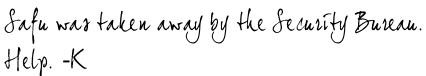
\includegraphics{Images/memo5.png}\\

He had not shown Shion yet. What was he to do with it? Nezumi was
suspended in his decision. He stood at a crossroads, unable to throw the
memo away, nor to pass it to Shion and turn his back on him, saying it
was none of his own business.

To be indecisive, to waver, and to be agitated ― he knew how dangerous
these were to him, almost painfully aware. Right or left; up or down;
fight or flight; abandon or protect ― the split second it took to make
the decision was the difference between life and death. He had never
once made the wrong choice. That was how he had survived up until now.

This memo is dangerous. Then, all he had to do was throw it away. Along
with the indecision that would no doubt endanger his life, it was for
the best to entomb it all in darkness.

He knew the correct answer. But why wasn't he complying with it? Why was
he taking the trouble, even paying a large sum of money, to have
information collected about the Correctional Facility? What the hell am
I doing?

His feet stopped.

Nezumi stood still, and trained his eyes onto the darkness. He was on a
slope sparsely populated with trees, a couple dozen metres away from his
underground abode.

"Who's there?" he spoke quietly. There was a dry rustling above him,
perhaps from a gust of wind that whistled through the bare branches. But
even more discreetly, there was a movement in the dark, the faint sound
of a step on the leaves.

"A little slow to notice, aren't ya?" There was a short bark of a laugh.
"Not like you, not like you at all. What were you daydreaming about?"

"Inukashi."

Inukashi's black hair and tan skin were convenient for blending into the
darkness. But it was careless of him not to have noticed his presence
until he had come this close. He was not himself today.

"Good thing it was only me. Who knows how many lives you'd need if you
were that dazed around anyone else, Eve." Inukashi called Nezumi by his
stage name, and gave another short laugh.

"Things aren't much safer with you around," Nezumi retorted. "Especially
if you're gonna be waiting at night to ambush me on the road." He took
half a step backwards. "What do you want, Inukashi? I find it hardly
likely you've been able to get the information this quickly."

Inukashi's tone of voice changed, and all sarcasm vanished from his
speech.

"We've got an emergency."

"Emergency?"

"Just now ― well, more like awhile ago ― Shion came to see me."

"Did he?" A jolt of unease raced through him, almost painfully.

"And not about his dog-washing job, either. He shoved a grey coat in my
face, and asked me if I got it from the Correctional Facility."

"Grey coat, huh... women's?"

"Yeah. It was ripped at the shoulder, but it was a fine piece of
clothing. It came from a used-clothes dealer I sold stuff to. Stuff I
got smuggled out of the Correctional Facility."

It must belong to that girl― Safu. Nezumi turned aside, and drew a
breath.

"So?"

"So?" Inukashi echoed incredulously. "You tell me. What's the script for
this act, huh, Nezumi? Shion says this coat belongs to his friend. Which
means his little friend is being kept prisoner in the Correctional
Facility. And earlier today, you gave me money to gather information
about the Correctional Facility. Don't tell me those aren't related ―
even a dog wouldn't fall for that lie. Are you planning to help Shion's
little friend out, is that what you're doing?"

Nezumi had no way to answer. He could neither affirm nor reject what
Inukashi had said.

"Of course not," Inukashi answered for him. "There's no way someone like
you would throw his life away to help a complete stranger."

"What makes you think I'm gonna die in the process?"

On the other end of the darkness, Inukashi sucked in a deep breath.

"Are you half-asleep? This is the Correctional Facility we're talking
about. By some lucky fluke, you might be able to sneak in. But there's
no way you'd make it out alive. Nezumi, don't get any funny ideas."

"Goodness gracious, are you worried about me? I'm shocked."

"I could care less about you," Inukashi snapped. "Whether one rat dies
or not isn't gonna make a difference. But what're you gonna do about
Shion, huh? Now he knows where his little friend's been taken. Being the
oblivious little boy he is, he probably thinks the Correctional Facility
is just some cushy Centre for Discipline, or whatever. He probably
figures all he has to do is hand in a Visitation Form to see his little
friend. If you don't stop him, the kid's gonna go. He's gonna go and ―
he's gonna get himself killed."

Inukashi fell silent, the darkness of the night seemed to deepen. Even
the wind was still ― the tree branches ceased to make even a faint
rustle.

"Is this what you've waited all this time to tell me?" Nezumi said
presently. "I ache to imagine what pains I must have put you through."

Nezumi stepped forward, and grabbed Inukashi by the shoulder before he
could slip away. As long as he had bearings on the other's presence, he
could more than easily predict all of his movements.

"It doesn't matter what Shion plans to do," Nezumi said quietly. "He's
not one of us, and it's none of our business."

"Then why the hell are you sniffing around behind his back?" Inukashi
replied accusingly. "Why do you need to gather information about the
Correctional Facility in secret?"

Nezumi stiffened his fingers and dug them harder into Inukashi's thin,
bony shoulder. Inukashi cried out in pain. Nezumi bent to bring his lips
near the other's ear.

"Don't stick your nose in things you have no business in," he whispered.
"You do the job you've been paid to do, and nothing else."

He let his hand go. Inukashi's small body swayed unsteadily.

"I only told Shion where the coat came from," he said. "I haven't told
him anything about what you've come to me for."

"Of course you haven't."

"Nezumi, Shion's gonna go alone," Inukashi said levelly. He feebly shook
the arm that was now numb all the way to his fingertips. "He thinks you
don't know anything about it. And he's gonna go alone, without telling
anyone. He's not gonna get you involved. You know that, right?"

"What makes you so sure? Are you Shion's Papa or something?"

"I don't have to be his Papa to know. You should know even better than
me what kind of person he is. That's why you're scuttling around in
secret, aren't you?"

"Shut up!" Nezumi had raised his voice in a snarl. His emotions whipped
about turbulently; his breathing came out irregular. Inukashi showed
almost no reaction.

"If he's so precious to you that you don't wanna lose him," Inukashi
said steadily, "protect him to the very end. And do whatever it takes to
protect him, you idiot, no matter how humiliating it is. You think you
can save face, huh? Keep it all hidden, and take care of it all on your
own? Stop fooling yourself."

"Inukashi!"

Inukashi sprang back a split second before Nezumi took a step forward.
Crouched on one knee, Inukashi laughed softly.

"You lose, Nezumi."

"What?"

"You've gotten yourself something you need to protect ― you lose. Those
are the rules in these parts. Better get to know them."

Nezumi kicked off the ground, and rounded in on Inukashi from the front.
He snared the other boy as he tried to get away, and pushed him to the
ground.

"What'd you say about losing?" he said fiercely. "That's enough bullshit
from you."

"I'm not bullshitting. Nezumi, if this was you a while ago, you wouldn't
have let yourself be provoked so easily. You wouldn't be walking around
at night lost in thought, either."

Let go, Inukashi said in an eerily calm voice. He got up, and heaved a
sigh.

"Still don't realize, Nezumi?"

"Huh?"

A sharp whistle tore through the air. While he whistled, Inukashi took
several steps backwards.

In the darkness from all directions, countless small red dots of flame
glinted as they emerged. It didn't take Nezumi long to realize that they
were dogs' eyes. Before he knew it, he was surrounded by a pack of them.
Not one of them raised so much as a growl as they formed a ring and
advanced on him.

"Those ones are trained guard-dogs. You're not gonna get the same deal
you did in the afternoon." Inukashi's voice was further away now. "You
stepped right into that ring without even realizing it. Definitely not a
mistake you'd normally make, Nezumi. But there's your weakness. Forget
Shion ― look at you, you can't even protect yourself."

After a moment of silence, a short command sliced the air.

"Get him!"

The dogs sprang up. Dozens of lithe and deadly bodies flew over Nezumi's
head and came down upon him from above as he sat crouched on the ground.
He sprang to his feet, and aimed a kick straight upwards.

A yelp.

One dog broke the silence with its voice, and crumpled to the ground.
Before Nezumi could catch his breath, another one kicked off the ground.
It sank its teeth into Nezumi's arm, which he had wrapped with his
superfibre cloth just in time. Nezumi swung his entire arm around and
battered the dog to the ground. He rose, and regained his posture with a
tree at his back.

"Inukashi, if you're gonna keep up this stupid game, I'm not gonna go
easy on you either." Nezumi drew his knife from its leather sheath. He
caught his breath, and counted the little red flames.

Four more.

"So you don't care if your precious dogs get their throats slit, huh?"
he called out.

Inukashi's voice answered from the same spot as before.

"Let's see you try. That was just a warm-up. They're not gonna be all
polite this time and come at you one by one. This time, they're coming
all at once."

Even before Inukashi had finished his sentence, Nezumi was lunging in
the direction of his voice. At the same time, a searing pain tore across
his shoulder.

"Out of the way!" He rammed the butt of the knife between the dog's
eyes. Along with the sound of tearing fabric, the black dog went rolling
across the ground behind him.

"Inukashi!" Nezumi yanked Inukashi by his long hair, and dragged him
down. He pinned him to the ground, and pressed the knife to his tan
throat.

"Back your dogs down, or else―"

Inukashi laughed shortly.

"Or else what? You gonna kill me?"

"If you wish it so," Nezumi said coolly.

"You think you can kill me, when you haven't even managed to kill a
single dog?"

This time, it was Nezumi who gave a soft laugh.

"But I don't have a spare knife today."

"What?"

"Dog's blood dulls the blade. I saved it and kept it clean for you."

Inukashi's body twitched.

"Hey, cut that out, you jerk," he said nervously. "You try and kill me ―
my dogs'll jump you all at once. They'll tear you to pieces."

"Oh, I don't know about that. You're their boss, right? I've heard
before that dogs lose their will to fight if their boss gets defeated."

"Th―That's not true― hey, really, cut it out. It's dangerous."

"Back your dogs down."

"Fine." Inukashi snapped his fingers. The dogs spun on their heels at
once, and disappeared into the darkness.

"I see. You've trained them well."

"Thanks for the compliment," Inukashi said sullenly. "Funny how it
doesn't seem to make me feel any better. So are you gonna get your heavy
ass off me or not? A love scene with you isn't exactly something I've
been itching to do lately."

"Don't worry," Nezumi said pleasantly, "it's the last thing I'd want to
be doing either. I wouldn't even do it if I got paid to on-stage."

After he had freed Inukashi and put away his knife, Nezumi posed his
question anew.

"What was all that for?"

Inukashi clucked his tongue while he brushed the leaves off his clothes.

"I took it upon myself to give you a private lesson."

"What?"

"The fact is, you're not as strong as you think. I just thought I'd
teach you that. You've got skill, though. Not many people can get that
far against me and my dogs."

"Why, thanks for the compliment. Funny how it's not making me feel
better."

"But you're not any superhuman or monster," Inukashi continued. "You're
just a human. And a man can only do so much by himself."

There was a dull pain in Nezumi's shoulder. Blood flowed in streams down
his arm.

A fleeting thought crossed Nezumi's mind. This was the same spot where
he had gotten the bullet wound which Shion had treated four years ago.

"Nezumi!"

He could hear Shion's voice calling him. The light of a lamp bobbed
nearer.

"Looks like the little lad has come to fetch you himself," Inukashi
snickered quietly. "Well, let me excuse myself then―" Then, somewhat
rushed, he added, "Nezumi, there's something weird going on inside No.
6."

"Weird?"

"I don't know the details. I've heard that there's some weird disease
going around, but I don't know for sure. I'm gonna look into it. And I'm
going to be getting information about the inside of the Correctional
Facility soon. It looks like things are starting to get busy for them
too. It's gonna get pretty interesting, I can smell it ― my dog's nose
is telling me. So―"

"So?"

"So count me in ― I'm gonna help you out."

Inukashi's hand reached out, and clapped Nezumi firmly on the shoulder.
A vicious pain shot through him. Nezumi groaned, and fell to his knees
with a hand pressed to his shoulder.

"See ya. I'll be in touch soon." Inukashi melted into the inky darkness
faster than his dogs had disappeared. As he faded, Shion's footsteps
approached nearer.

"Nezumi, did something happen?"

Shion held the lamp up to Nezumi as he got to his feet. His eyes widened
in alarm.

"What happened to you? You're bleeding!"

"I got attacked by a dog."

"A dog? Why?"

"It was just some mongrel. I guess it thought I was a cute little bunny
rabbit. What are you doing here?"

Hamlet poked its head out from Shion's sweater pocket.

"He came to get me," Shion said. "I thought something might've happened
to you."

"So you came to help. With one lamp."

"Yeah." Shion brought the lamp closer to Nezumi's wound, and furrowed
his brow.

"We have to get this treated. Let's go home. Can you walk?"

"Of course."

Shion's slipped a hand under Nezumi's armpit, as if to support him.
Nezumi brushed him away, and began to walk ahead. His shoulder throbbed
painfully. But he wasn't about to cling onto the hand that was extended
to him. If he learned to lean on someone, he would never be able to walk
on his own again. The helping hand was always fickle, and disappeared
just as suddenly as it was offered. That was how things were.

Once they returned to their underground room, Shion sprang into action,
briskly taking the appropriate steps. He checked the wound, cleaned, and
disinfected it.

"You gonna sew it up again?"

"The wound isn't that bad this time, unfortunately," Shion said, in a
rare rueful grin as he closed the emergency kit. "Freaked out a bit,
didn't you, Nezumi? Thought you'd go through the same thing as four
years ago?"

"'A bit' is an overstatement. With you, I feel like I'd end up with
stitches for a bug bite."

"How rude," Shion smiled. "I still think the treatment I gave you four
years ago was the appropriate thing to do."

Four years ago, on that stormy night ― yes, on the night he had first
met Shion ― No. 6 had been in the midst of a hurricane. He still
remembered, ever so vividly, the window flung open as if to invite him
in; twelve-year-old Shion as he poked his face out; You're hurt, aren't
you? I'll treat your wound' ― words that he had never expected; the
satisfied smile that had spread over Shion's face the moment he had
completed the suture; the sweetness of the cocoa; the delicious taste of
the cherry cake; the comfort of the bed; the sound of quiet, slumbering
breaths right beside him as he awoke the next morning ― he couldn't
forget any of it, no matter how hard he tried. Even when he tried to
discard it, he could never quite bring himself to.

Each and every miraculous occurrence of that night still remained with
him as tangible sensations, never fading in the least over the four
years until now.

Did people call them memories? A mental record? Or did they call it
fate?

It was easy enough to laugh at people, calling them indulgent and weak,
when they accepted others unconditionally and tried to save them.
Indeed, as a result of taking Nezumi in, Shion had lost almost all of
his privileges and fortune.

How much easier things would have been if he was able to dismiss Shion
with a condescending laugh, this naive boy, this petri-dish elite who
had grown up oblivious to society. But it was too bitter to laugh at and
be done with. It was too vivid to forget. And to throw away, it was much
too heavy.

"Shion."

"Hm?"

"Do you really think so?"

Shion's hands stopped in the middle of winding a bandage.

"Four years ago. Do you really think it was the appropriate thing to
do?"

"Well, we were in pretty limited surroundings," Shion said slowly. "Back
then, though, that would have been the most I could do. Now, maybe I
would be able to sew it up a bit better." The long fingers of his
deft-looking hands moved as nimbly as they looked, winding the bandage
tightly and neatly.

"Not just about my injury. About the whole night."

After he had knotted the ends of the bandage with care, Shion studied
Nezumi's eyes.

"Your life turned 180 degrees that night. Can you still say, even now,
that what you did wasn't a mistake?"

"Yeah." His answer was so prompt, Nezumi was caught off-guard.

"You don't regret it?"

"No."

"Not even a bit?"

"No."

"Why?"

"Nezumi, I don't really understand what you're trying to ask. But I've
done a little thinking myself since moving to Lost Town. I wondered, if
I were to go back in time, and return to that night four years ago ― if
I were to return to before I met you, what would I do?"

Shion smiled sheepishly, and pushed the emergency kit to the back of the
shelf.

"I thought about it, over and over again. And every time, there was only
one answer. No matter how many times I'd return to that night, I'd do
the same thing again. I'd open the window, and wait for you."

"Even if you knew that your own ruin would be waiting beyond it?"

"But there wasn't any ruin," Shion replied softly. "I don't think my
being here like this has ruined me at all. Right, Cravat?"

The small brown mouse nodded from its perch atop a stack of books.

"That one's Hamlet, isn't it?"

"Hamlet's sleeping on the bed."

"Oh. Right. ― Geez, you had to go giving them stupid names, now it's
more confusing than before."

"The poor guys deserve names, it's the least you can do. Both of them
are smart and courageous. Like Hamlet today, when he let me know that
you were in danger."

"Well, he went to the wrong person. Even if you showed up, you wouldn't
be much help. It was alright this time because I'd already chased the
dogs away, but if I hadn't, you'd probably be the one sitting there with
a gaping wound."

"Yeah, well ― I guess you're right about that one."

Nezumi stood up, and grabbed Shion by the arm.

"Never do something like that again, you hear me? Whatever happens,
don't flatter yourself and think you can be any help to me."

Shion stared back at him with unblinking eyes. Nezumi lifted his chin,
and clenched his jaw.

"You're powerless, you remember that. You don't have the skill or the
mentality it takes to fight. You're like a chick that's fallen out of
its nest. You'd just chirp-chirp-chirp until you're eaten by a fox. So
do yourself a favour, and don't go walking into danger's path. Don't do
it, ever. Use your head. Put your so-called gifted brain into motion,
full-throttle, and use your judgment to assess the situation. Geez, I
don't know what the hell you were thinking, running out into the
darkness without even carrying a weapon."

"I wasn't."

"What?"

"I wasn't thinking at all, of the situation, or of danger. I was already
running before I could stop to think."

"That's why I'm saying, Shion, next time, don't ever do something as
foolish or reckless."

"Then what should I do?"

"Don't do anything. There's nothing you could do anyway. Pull a blanket
over your head or something, and stay quiet."

Shion dropped his gaze, and shook his head.

"I can't do that," he said quietly. "I can't stay there and sit still
when I know you're in trouble. I would've burst outside either way."

"You'd just be a hindrance."

"That's harsh," Shion said softly.

"It's the truth."

"Nezumi ― you're right," he relented. "I'm useless. I don't know how to
fight, and I would never be able to bring myself to hurt anyone."

"Yeah, and as a soldier, that would put you in the lowest rank. No ―
actually, you'd be a write-off. So don't even think about fighting. You
don't have the mental leverage to be worrying about other people. You
can't even protect yourself. So don't do anything. I'm begging you, just
don't go near any dangerous places."

What the hell am I saying?

Nezumi clenched his jaw again.

What was he saying? What was he doing, getting serious about this? Was
he that bent on stopping Shion?

Shion's gonna go alone.

Inukashi's low voice echoed in his ears.

Yes, Shion would probably go alone. He'd set out to a place with less
than one in a million chances of returning alive, and he'd go alone,
without begging for my help, without even telling me. He would go
silently, not knowing anything about fighting, not knowing the pain of
shedding blood or the chilling horrors of murderous intent. The useless,
big-headed, oblivious idiot.

"But it's not about reasoning," Shion said quietly, puncturing the
silence.

"Huh? Did you say something?"

"It's not about reasoning, Nezumi. I know very well in my head that even
if I were to show up, I wouldn't be of any help to you ― I wouldn't be
able to save you. I know."

"Good for you. The grey matter in your head is about the only thing you
can boast about, anyway. And if your head knows, then take its advice."

"No."

Shion pursed his lips firmly, his expression defiant. It was the face of
one whose willpower ran strong and deep. It was Nezumi's first time
seeing Shion with a face like this.

"It's not about reasoning!" Shion said heatedly. "Back there, when
Hamlet came to call me, I was scared. I thought something had happened
to you. I thought you were going to die. Are you telling me I should've
just stopped and calculated in my head? Figured that it wouldn't do any
good if I went anyway, and just sat still? I could never do that. How
could I? How could I be cool and calm and think about whether I have or
don't have the strength, whether I can or can't help you? How could
anyone? Idiot!"

It was his second time being called an idiot by Shion. Both times,
Nezumi wasn't able to predict Shion's explosion of anger. The first
time, Nezumi had told Shion, 'Don't cry for other people. Don't get into
fights for other people. Fight and cry only for yourself.' Shion had
said that he didn't understand. It was true, he hadn't understood. For
this time, again, Shion had burst out into the darkness for a stranger.
Casting aside the reason which warned him of the risks, he had gone
running into the darkness. It was dangerous. Very dangerous. Nezumi had
been prepared for Shion to become shackles that bound his ankles. But
there was also the opposite. There was a possibility that he himself
would become the fetters that bound Shion's wrists.

This is why―

Nezumi averted his gaze from the boy in front of him.

This is why humans are troublesome. The more you involve yourself with
them, the tighter the shackles become. They hinder free movement. It
becomes harder to live only for yourself. Maybe we should never have
met. Maybe one day, Shion, you'd come to think so.

Shion's shoulders rose and fell as he took a deep breath. He stuck his
lip out in a disgruntled manner.

"Nezumi, why aren't you saying anything?"

"No reason."

"Go on and laugh if you want to. You probably just think it's all
gibberish from someone who doesn't know a thing about the world, right?
Fine. Laugh to your heart's content. Go on, laugh."

"Wait a minute, Shion," Nezumi said hastily, "it's not like I'm mocking
you. I just, well... I'm just saying it's dangerous to jump into danger
like that, without thinking about―"

"I know that!" Shion said hotly. "But I couldn't help it, alright, I was
worried sick. Or am I not even allowed to worry about you? Don't I even
have the right to be worried?"

"The right? Shion, you're not making sense."

"You're the one making me talk like this!"

Shion's fist pounded the bookcase. A mound of books collapsed. Cravat
gave an alarmed screech, and skittered into the folds of Nezumi's
clothes.

Shion blinked, and his cheeks flushed. He bent to pick up the books, and
mumbled an apology in a subdued voice.

"I'm sorry, I just ― I didn't mean to yell."

"I don't mind," Nezumi said lightly. "I must say it was quite alluring
to see you all worked up like that. Something I'd like to be treated to
again once in a while."

"It seems like I'm always worked up when I'm with you," Shion sighed.
"I'm surprised at how emotional I can get sometimes."

"You've always been an emotional person. You always choose feeling over
reason, and you're not ashamed to be truthful to your emotions. Four
years ago, it was the same. Even when you were a candidate for the elite
echelons of No. 6, you still obeyed your emotions and took me in."

"Yeah... obeyed my emotions..." he said pensively. "I guess you're
right."

Shion stacked the books neatly, and exhaled.

"But you know, Nezumi, I really don't regret it. I'm still glad that I
didn't turn my back on my feelings that night."

"I know."

"Huh?"

"I know you don't regret a single bit of what you did. I just asked on a
whim. I guess I was probably bored, or something."

He brought a hand to his shoulder. The bandages, which were old and
worn, and would have lost all elasticity by now, wrapped themselves
tightly around his shoulder and arm joint, and showed no signs of
loosening.

"I wouldn't have been able to dress my wound this well," Nezumi said
reflectively. "You might not be able to fight, but you can probably
treat people. Everyone has something. And probably―"

"Probably?"

"No, never mind. Say, I'm hungry, aren't you?"

Shion gazed at Nezumi, and gave a gentle smile.

"There's bread and meat on the table. Some stuff happened, and there's
only a little bit left, but it should be enough for dinner."

"What about you?"

"I'm going to sleep. Your wound is probably gonna keep you up tonight,
so you can have the bed to yourself. I'll sleep on the floor."

"How kind of you."

"Nezumi."

"Hm?"

"If I hadn't met you, I probably would never have realized what kind of
person I was, huh?"

"Why're you bringing this up now?"

Shion drew nearer to Nezumi as he sat in his chair, and looked him
straight in the eye.

"I would have grown up into a mild, rational, obedient adult, without
even knowing there were so many emotions inside of me. I would never
have known what it was like to cry, or get angry, or feel resistance
toward something. I met you, and I realized how much abundance I had.
And I'm proud that I know now."

Shion clipped his words, and hesitantly lowered his eyes.

"I'm glad I met you."

It came out as a whisper that he could barely catch. Shion bent down,
his eyes still lowered. His lips brushed lightly against Nezumi's.

A book fell somewhere with a soft whump.

As Shion lifted his face again, Nezumi spoke.

"Not a thank-you kiss, is it?"

"It's a good-night kiss."

"Good-night, huh."

"I'm going to be shearing the dogs tomorrow," Shion said. "There are a
whole lot of them with long fur. Inukashi just leaves them, so their fur
gets all tangled and they're starting to get skin inflammation."

"I just got bitten by a dog, alright? I don't care if they have short
fur or long fur, I don't even want to hear about dogs right now."

Shion laughed out loud, and gave a casual wave of his hand.

"Good night, then."

"Yeah. Sweet dreams."

"You too."

Shion disappeared into the shadows of the books. Cravat crawled out from
Nezumi's clothes and scampered after him, perhaps intending to sleep
with him too.

"Good-night kiss, huh."

Nezumi traced his lips with his fingers, and slumped back in his chair.

"Some liar you are."

His gnawing hunger, exhaustion, and throbbing pain ebbed away. In its
place, something welled up from deep within. Sadness, loneliness ― it
wasn't quite either. What was it? A hot bead rolled down his cheek. It
took him a while to understand that they were tears. He had long
forgotten what it was like to cry.

It tasted salty, like over-salted soup.

Nezumi propped his knees up and put his head down on them. Slowly, he
swallowed the tears that seeped into his mouth.

\hypertarget{index_split_088.htmlux5cux23calibre_pb_111}{}

\protect\hypertarget{index_split_108.html}{}{}

\hypertarget{index_split_108.htmlux5cux23calibre_pb_0}{}

\hypertarget{index_split_108.htmlux5cux23calibre_toc_6}{%
\subsection{CHAPTER 5}\label{index_split_108.htmlux5cux23calibre_toc_6}}

\subsubsection{In Falsity's Company}

In days of old, the Buddha

was but a mortal;

in the end, we ourselves

will be buddhas too.

How grievous that distinctions

must separate those

who are alike in sharing

the Buddha-nature!

- Tales of Heike: Giou {[}1{]}

Shion slowly raised himself off the floor.

Only a few dying embers remained in the heater, and the room was
freezing cold. Cravat, who had been curled up against Shion's body,
raised his head and chirruped softly.

"Shh―" Shion drew his blanket around the little mouse. "Here, you sleep
in this. Just please don't make any noise, okay?"

Shion had gotten so used to this room that he could find his way even in
the dark. He padded stealthily to the door. He unlatched it, and before
opening it, he turned back again. He listened carefully. There was not a
noise.

It looked like the pain from Nezumi's wound hadn't kept him from
sleeping. I guess a wound that small wouldn't be enough to keep him
awake. There were so many things he still needed to tell Nezumi. The joy
of meeting him, the gratitude for everything he had done for him, and
the profound respect he had for him ― Shion had not been able to get any
of these adequately across.

I'm glad I met you.

That was all I was able to say.

Shion inhaled the air of the room deeply, just once, before quietly
opening the door.

* * *

The lamp flashed, signalling a call from a direct extension to City
Hall. The man lifted his face from the research documents he had been
perusing, and lightly clucked his tongue in irritation. The document,
which had been printed decades ago on paper, was very intriguing, and he
wished to read a little further. But the lamp was flashing red,
signalling an emergency situation. The man clucked his tongue again, and
put the documents away in a folder.

When he pressed the switch, the familiar face of a man appeared
on-screen. He was a man who used to be called Fennec.

Fennec ― the desert fox. Who was it that had first started calling him
that?

"What's the matter, Fennec?"

"We have an emergency. Two samples have been brought into the Central
Hospital."

"Something the matter with that?"

"Both of them aren't registered as representative samples in the data."

"What?"

"They're different from the samples you've requested from us. Things are
happening on their own, outside of our control."

"Perhaps it's too early to conclude that they're samples. Couldn't
something else be the cause?"

Fennec shook his head. The screen promptly changed to another image. An
audio clip read out the two bodies' personal information.

Name, age, address, occupation, history of illness, physical
measurements, citizenship number...

A man and a woman. Two bodies. Both their faces were contorted in
suffering, and were aged and shrivelled. It if weren't for their facial
expressions, their cause of death would easily have passed as old age.
But the documented age of one of them was in the twenties, the other in
his late thirties.

"You're right, they must have done it," the man muttered. The screen
flickered again, and Fennec's scowl was displayed largely. The man
exhaled quietly.

"...What could this all mean?"

"I think I would like to know that!" Fennec raised his voice, and his
ears twitched indignantly. Ah, yes. This was a habit of his. Since he
was young, he had always had the habit of twitching his ears when his
emotions were agitated. That was why he was called Fennec. A fennec fox
was a small fox with the longest ears of its kind, reaching up to
fifteen centimetres.

"But how could something unexpected like this happen?" Fennec continued.
"I don't believe it. What's going on?"

"Something must have gone wrong somewhere," the man answered. "But it's
insignificant. It's nothing you should be worried about."

Fennec's throat contracted as he swallowed at the man's words.

"Are you sure?"

"Of course."

"You have the highest responsibility in this project, you know."

"Not officially," the man added. "Well, but then again, nothing about
this project has been publicized officially."

"But if this succeeds, then No. 6's City Project will finally be perfect
and complete. Right?"

"Yes."

"Then even minor slip-ups can't be permitted."

"I know. I'll launch an investigation immediately looking into the
cause. I want you to send the bodies over to the Special Autopsies Room,
Section V."

"I've already got it underway."

"Then I'll get to work straightaway."

"Please do. I'll be waiting for the report."

"Roger."

"Oh, yes," Fennec added. "Once this mess has quieted down somewhat, I'm
planning another clean-up."

"Clean-up? That's something I haven't heard in a long time. Say, it's
almost the Holy Celebration, isn't it?"

"Yes, the same reverent day is coming again. If you need any for your
experiments, I can arrange for as many as you need. What say you?"

"I am most humbled by the kind considerations of His Excellency."

"None of that embellished formality, if you will."

"But you'll eventually become the absolute ruler of this land," the man
said. "The one and only King. I'd have to start calling you Your
Highness."

"And what would you have me call you?"

"I'll stay as I am. If I'm still provided with the same top-notch
research facilities and environment as I am now, then I have nothing
more to ask."

"Sparse in your wants as always, I see. Then I trust you'll have the
work done."

The screen silently went blank. The man let his gaze flit over the
documents he had only partially read. Unfortunately, it looked like he
would not be able to read through the rest of it today.

They were documents concerning a species of ants called Eciton
burchelli, which inhabited Central and South Americas. These ants, which
formed colonies numbering up to 500,000, did not live in one static
place, but instead repeated cycles of temporary encampment and migration
until their life was spent. There was only one queen ant that reigned
over the colony of 500,000. But the queen's sole purpose in the colony
was to lay eggs, and she was not necessarily in control of its members.
Warrior ants and worker ants, large and small, all moved accordingly to
their instinct, and as a result, the colony functioned seamlessly as if
they were governed by a great common intellect.

Ants, and bees too, had created the ideal social system.

There was no way that humans could not do what insects already did. Each
would obediently fill his role. Without thinking, without being
interrupted by suspicions, they would take to their task. Brains were
unnecessary. Souls were of no use.

A colony of 500,000, and a single one to reign over all.

You say I'm sparse in my wants, do you? You're right, Fennec, I desire
nothing. I have no need for desire. I never have to suffer from being
dominated by my desires, like you do.

The man smiled discreetly, and pushed the button for the elevator
leading directly to the Special Autopsies Room.

* * *

A frost had fallen. The frozen grass underneath his shoes made crunching
sounds as he trod over them. When the sun rose, the frost would sparkle
white, and the barren expanse would be enveloped in light for a fleeting
instant. But it was too early ― the sun had yet to rise for a while
longer. Shion stopped in his tracks, and lifted his face to the northern
sky. He wanted to reach the Correctional Facility before dawn. He had no
idea what he would do once he arrived. But he had to go. It was all he
could think about. Why had Safu been impounded in the Correctional
Facility, when she was supposed to be abroad? Was it in connection with
him? If it was, then would Karan's safety also be compromised?
Uncertainty and fretful misgivings coursed through his body, blocked his
airway, and pressed against his heart. He didn't want to lose anyone,
neither his mother, Safu, nor Nezumi. He would do anything to protect
them. But he was frustrated at himself for not being able to come up
with how he would do so.

Even now, as he was walking, Safu was probably alone and frightened. He
had to do something. He had to save her and get her out. But what was he
to do? How could he―

Cheep-cheep.

A soft cry. His feet stopped. His eyes, which had gotten used to the
darkness, trained on a small rodent poking its face out from the grass.

"Cravat?"

He scooped up the tiny mouse in his hands.

"Did you follow me out here? Go home, you shouldn't be―" He realized as
soon as he had said it out loud, that this mouse was not Cravat. It
wasn't Hamlet, either. It wasn't even alive. This mouse carried no sign
of the warmth that living animals did.

"This is― a robot―?"

"He's the navigator." There was a voice behind him. He didn't have to
turn around to know who the voice belonged to. Shion took a few measured
breaths, and slowly turned his body around.

Nezumi was also approaching him slowly. He plucked the miniscule robot
from Shion's hands, and tossed it into a pouch.

"It's a simple navigator robot with three-dimensional mapping functions.
It was warning you because you were going in the wrong direction."

"The wrong direction―"

"Weren't you going to Inukashi's place? You were gonna give those
long-haired dogs a trim because their skin was getting inflamed, weren't
you? Leaving awfully early, huh? How diligent of you. But this isn't the
way."

Shion inhaled the frigid air of dawn yet to come.

"This has nothing to do with you," he said bitingly. "It's none of your
business what I do, or where I go. I'm sick and tired of you trying to
act like my guardian. I'm not a helpless baby. Just leave me alone. You
know what," he said, "it's enough. If you still think of four years ago
as a debt, then let me tell you now, it's paid back. You've given more
than enough already. From now on, I'm going to be free. I'm going to do
as I please, without being strapped down by you. That's my decision, so
don't get in my way."

He ran out of breath, and lapsed into silence. It was too dark to see
the expression on Nezumi's face. His shadowy figure shifted slightly,
and he could hear a soft applause.

"That's quite some recitation for an amateur. Maybe you do have a talent
for acting after all. Certainly better than yesterday's kiss, at least."

"Nezumi, what―"

He thought he saw Nezumi's right hand swing upwards, and then a hard
blow struck his cheek. Shion staggered, and fell backwards. The taste of
blood spread inside his mouth.

"―what was―!"

"Get yourself up if you have the time to be asking questions. The next
one's coming."

The tip of Nezumi's boot swung straight toward him. Shion instinctively
rolled to the side.

"Don't just stop there. Keep moving, keep the flow."

A kick landed firmly in Shion's ribs. His breath caught in his throat.
He blindly grasped at a handful of pebbles that littered the grassy
patch.

"Don't close your eyes. Don't look away from your opponent's attacks.
Move!"

Shion twisted around to whip the pebbles at Nezumi, and at the same
time, kicked off the ground and tried to ram into him with his shoulder.
His feet were swept from under him, and he was slammed to the ground.
This time, he could not get up again. He could see the stars. The stars
that scattered across the sky yet untouched by dawn twinkled almost
frightfully bright.

He was grabbed by the arm, and pulled up off the ground.

"Shion, this is punishment."

"Punishment for what?"

"You lied to me."

"Well―"

"You'll admit that, won't you?"

"Yeah... I guess."

"Your second crime. You belittled me."

"I never did that."

"Lying to someone means you're belittling him. Did you think I would
fall for your lame excuse? If that's not an insult to me, I don't know
what the hell is."

"It was my best attempt," Shion protested feebly.

"Well, you'd make a horrible politician or writer, seeing how you can't
even conceive a realistic lie."

"Was it that bad?"

"Atrocious. But this is what pisses me off the most, Shion―"

"Yeah?"

"That you must've figured I was some brat who couldn't tell one kind of
kiss from the other. What good-night kiss, huh? Bullshit."

Nezumi knelt in front of Shion, and gripped his collar tightly.

"You hear me? Never give me a farewell kiss again. Ever."

"I'm sorry."

"And never lie to me again."

"I won't."

"Swear it."

"I swear."

The hand released him. Nezumi settled into a sitting position, and
looked up at the heavens.

"I've heard there are strange things happening inside No. 6."

"Strange?"

"I don't know the details, but Inukashi is gathering information for me.
If we do it well, maybe we can use old man Rikiga and get some
information through his customers, too. And it looks like stuff is going
on in the Correctional Facility as well. There's commotion happening
both inside and outside of No. 6 at the same time. A little weird, don't
you think?"

"Correctional Facility? Nezumi, are you saying―"

"Your important friend, or whatever ― you called her your best friend,
right? ― I've known about her for a while."

He handed Karan's memo to Shion. Shion's fingers began to tremble after
he had read the note.

"Your Mama is safe for now. I'm not so sure about your bestie. But don't
panic. Right now, we have to gather all the information we can and set
down a plan. Inukashi says he'll help. This is all preparation so that
we can infiltrate the Correctional Facility as soon as possible.
Understand? We're not going in there to get killed. We're going in there
to save her. Be calm."

Shion nodded.

"So I've finally dragged you into the mess, too."

"It's not your fault. Inukashi says he smells something, and frankly, I
have my own suspicions too. Why would they need to imprison a precious
member of their elite? There's a chance that it might have to do with
the wasp incidents."

"The parasite wasps, huh... but they're not active this time of year."

"That's why something must've happened, something unexpected. And if it
has, then it might be worth risking the danger. Whatever the case,
whenever Inukashi gets into contact with me is when we make our next
move. Until then, we have to gather our own information and start making
preparations."

Nezumi stood up, and spoke in a beautiful voice that rang out
crystalline.

"Cheer up. Things will work out. We'll make them work out."

"Thanks. You've saved me again."

"Things are just getting started."

Shion stood up as well, and called the name of the boy who stood beside
him.

"Nezumi."

"Hm?"

"Mind if I―"

"Huh? What?"

As Nezumi turned to peer inquisitively at him, Shion slapped him across
the face as hard as he could. Nezumi, of course, didn't so much as
stagger ― but he was certainly startled. After drawing a breath, he
yelled,

"―the hell was that for?"

"It's punishment."

"Punishment?"

"You hid things from me. You didn't even mention a word to me about this
memo."

"What would telling you do, anyway? I couldn't have you wandering off by
yourself like you did tonight. I did you a favour and looked out for
you. Or what, are you saying I don't have the right to be worried about
― wait, I've heard this line somewhere before."

"Worrying about me and hiding things from me are two completely
different issues. It's not like I want to be sheltered by you. I don't
want to coast along living the easy life, always being protected by you.
I want―"

Shion softly clenched his fingers around his palm, on which he could
still feel the sensation of Nezumi's cheek.

"I want to be equals with you."

Nezumi hunched his shoulders, and lifted his right hand in a pledge.

"I admit my mistake. I won't do it again."

"Do you swear it?"

"I swear herewith upon my battered cheek."

In the distance, a cock was crowing. Even in this darkness, it could
sense the coming of dawn, and heralded it loudly and shrilly. In
moments, the eastern skies would lighten, and the light of the sun would
wipe the darkness away. The first day of their battle was about to
begin.

* * *

Safu was trying to wake up. She could feel her consciousness gradually
beginning to return. But her physical sensations were still murky.

Where am I?

What am I doing here?

Am I dreaming?

I have to remember.

Remember what?

My very precious person.

Precious person.

"Safu."

She could hear a voice very closeby, a man's voice.

No.

It's not this voice.

The voice I'm waiting for

isn't this voice.

"How are you feeling? I daresay you must be feeling a little different
from what you're used to? But you'll get used to it in no time. I hope
you like this special suite. It's the best you could ask for, and it's
especially for you, Safu."

I don't like this voice.

Don't call my name.

Don't call my name

with that voice.

"Safu, you are quite beautiful. Even more than I imagined. Beautiful,
indeed. I'm very satisfied."

I don't like this voice, and

I don't like this smell.

It smells like ― blood.

The smell of blood.

"I'm rather busy today. I'll come again, Safu. You should relax and rest
a little as well."

The footsteps faded away, and so did the stench of blood. She was
relieved.

But why

Why is everything so

hazy?

But I

From the margins of her consciousness, which was not completely
recovered yet, a flash of a figure emerged vividly.

Those eyes, those nails, that mouth, the faraway gaze, the energetic
smile, or that clouded expression, the long fingers ― and oh, she could
hear his voice.

"I always thought of you as a friend."

He was always such a child. He had never even realized her feelings for
him. But there he was, desperately searching and yearning for someone
else. She had loved that childish, but intent soul of his. She had loved
him like she could love no other. Even now―

She was fading out of consciousness. The darkness gently draped over
her.

I'll never see you again....

Shion.

Shion spent the majority of the day taking care of the dogs. There had
been no sign of Inukashi in the morning, so Shion had had to prepare
food for and groom ten some-odd dogs all by himself. He had barely any
time to rest, but he didn't feel the labour to be onerous. On the
contrary, he was actually grateful for it. Immersed in his work, he
could forget his agitation, even for a short while.

Don't rush, and wait patiently. Act calmly.

Nezumi's words were certainly persuasive, and he had no choice but to
nod his head, but still he couldn't help his agitation. He could not
remain calm.

Even while I'm going about this now, Safu is...

Every time the thought crossed his mind, his emotions would be thrown
into disarray, he would panic, and he would bite his lip until it bled.

A dog whined forlornly. It was one from a litter of puppies that had
been born at the start of fall. Shion realized he had been staring off
into space in the middle of making their meal.

"Oh, sorry."

He hastily scooped the stewed leftovers into their food bowls. The
puppies fiercely wagged their identical tails as they dipped their faces
into the food. In the kind of circumstances where even humans starved to
death, Inukashi managed to provide for his dogs with enough so that they
did not starve.

The leftover food was shipped into the ruins in the middle of the night,
and was sorted into food for humans, which would be shipped to the
market, and the rest, which was used for dog feed. Shion finally knew
where it came from now. Inukashi was probably tracing this route.
Nezumi, too, had disappeared in an early part of the morning.

What could he do?

The more he thought about it, the more he came face-to-face with his own
powerlessness. It agitated him. He could not stay calm. And he would
bite his lip again, and try to endure.

There was a warm sensation on the back of his hand. He looked down to
see a puppy intently licking his hand. Cravat poked his head out from
the breast-pocket of his sweater, and ducked back inside again.

He wanted to show Safu this puppy, and this little mouse. He wanted to
let her touch them, and let her feel the warmth of their little tongues
and bodies.

Safu was dear to him. She was precious to him. But it was different from
the amorous sense ― it was more serene, more deeply connected. He loved
her like family, like a close friend. Whatever kind of love it was made
no change to the fact that he cared about her.

He closed his eyes. He called her name.

Safu.

"You want me to co-operate with you?" Rikiga made a clearly distasteful
expression.

"Yeah," Nezumi answered. "I want you to glean information from your
customers." Nezumi seated himself snugly into the chair, and put his
feet up on the table.

"Information? You mean about the Holy City?"

"Yeah."

"What's in it for me?"

"Enormous riches."

Rikiga stood up, and strode over to Nezumi. They were in a room of the
building Rikiga used as his workplace. It was a room littered with
magazines and empty bottles, and it reeked of alcohol. Looking down at
Nezumi, Rikiga twisted his mouth in a scowl.

"Some long legs you've got, huh. Showing off?"

"What an honour to be complimented by you. These are the money-makers, I
gotta keep them in shape."

Rikiga's hand rapped sharply on the pair of legs flung out onto the
table.

"Get your feet off my table. It's obvious what kind of upbringing you've
had," he said scornfully. "Don't even know your basic manners, do you?"

"I use my manners with people who deserve them."

"Not to mention your filthy language," Rikiga continued. "And this
favour you're asking for, is this some kind of act? Are you practicing
for some new part you've got?"

"It's a real issue."

"A real issue, huh. Enormous riches, you say? Ridiculous."

Nezumi glanced at Rikiga's face, and flashed a faint smile.

"What's wrong?" he said. "This is about making a fortune ― you love this
kind of stuff. Not feeling up for it?"

"What makes you think I'm gonna believe what some third-rate, fraud of
an actor tells me?"

"Then who would you listen to? Shion?"

Rikiga's gaze wavered.

"Shion? Does Shion have something to do with this?"

"He has a lot to do with it."

"Did you get him involved, Eve?"

"No. Shion sowed the seeds, they're just growing in my yard."

"What do you mean?"

"If you agree to help me, I'll tell you."

"Spit it out."

"First, I want you to show me your customers' stats. When's the next
time a high official from No. 6 is gonna come to have a good time? I
want to know his name, and position."

Rikiga exhaled shortly, and folded his arms.

"Eve, how old are you?"

"Younger than you, old man."

"You must be young enough to be my son. I've been meaning to say this
for a while, but a brat like you has no right to look down on adults
like this. You're bound to serve the consequences."

With his eye still trained on Nezumi, Rikiga called out, "Conk," in a
loud voice. The door to the next room opened, and a large man walked in.

"He's my new bodyguard," Rikiga said. "Just got him hired. He used to be
a wrestler, and people used to bet on the matches. He's nearly killed
several people with his bare hands. On the ring, and off the ring too."

The man silently gazed down at Nezumi. He was so large, he made the
dirty room seem a size smaller just by walking in.

"Conk, I want you to give this little prince here a proper welcome. You
don't have to kill him. Just enough so that he'd never be able to make
another smart comeback again."

"Huh?" Conk stuttered. "Uh―"

"Don't 'uh' me, I'm telling you to teach this kid what a punch from a
real adult is like," Rikiga said irritably.

Conk licked his lips, and took a step forward. And another step. Nezumi
stood up. Rikiga smiled contemptuously.

"This is the punishment you deserve, Eve. The full extent of it."

Conk's feet stopped.

"Eve ― is it really you, Eve?"

Nezumi smiled, and proffered his hand in a delicate gesture. His sensual
smile made even Rikiga blink.

"So your name is Conk? Pleased to meet you, Conk. Thank you for always
coming to see me on stage. I would never have dreamt that I'd be able to
meet you here. I'm so happy."

"Oh ― Eve, me too."

Conk blushed crimson, and gently clasped the hand that was offered to
him.

"I've always been a fan of yours ― I've seen almost all of your
performances―"

"I know. You stood out, so I always knew whenever you came to my shows.
You'd even send me gifts sometimes. I've always wanted to thank you
directly."

"Really? You ― you could really tell when ― when I―"

"Of course. And last time, you even cried. I was watching you from
on-stage, too, you know."

"Watching? You were watching me?"

"Watching you."

"Eve ― I don't know how to say ― I ―"

"You're overwhelmed?"

"Yeah, overwhelmed. With happiness. I've never been so happy. I feel
like I'm floating on air."

"Thank you, Conk," Nezumi said pleasantly. "And I hate to disturb you,
but I'd like to have a nice, long talk with Rikiga-san. Would you be so
kind and pour me a cup of coffee?"

"Of course. Anything to eat?"

"That would be nice. Do you have meat pie, by any chance?"

"Yeah. I'll bring it rightaway."

Conk disappeared into the next room with amazing swiftness for his
stature. Rikiga shook his head.

"Coffee and pie, huh? That stuff is all mine, you know," Rikiga
grumbled.

"Don't complain, or he'd probably punch you. You said so yourself.
Ex-wrestler. Nearly killed several people. Right?"

"I can see why his wife kicked him out of the house," Rikiga said
bitterly. "He's completely useless when you need him the most."

"He's a good guy. Probably makes excellent coffee."

Rikiga clucked his tongue three times.

"That's quite something, Eve. Not only can you handle a knife, can you
also use sex appeal to your advantage too?"

"Both make good weapons."

"Then use that weapon you've got."

Nezumi lowered himself into a chair and crossed his legs.

"Eve, you're no rat," Rikiga continued. "You're a cunning white demon
fox, great at manipulating people. Now, I don't know how many tails
you've got, but I've got a man who likes that kind of thing. He's an
elite, works at the Central Administration Bureau. He's my best
customer."

"Does that mean you're co-operating with me?" Nezumi's face was sombre.
Rikiga's face was also grave.

"I've also heard that there's been commotion recently inside No. 6."

"News reaches you quick, huh. I'm impressed."

"Don't try to flatter me with things you don't mean. Staying on top of
the news is what keeps my business running. But really," he said
bemusedly. "This is the first time I've heard about anything out-of-line
coming from that place. And that's how many decades since the Holy City
came to be? It's probably about time things started fraying at the
seams. And if that's the case, then I want to know more. I'm still
concerned about these things, Eve. And if Shion's involved ― then I
don't want to turn a blind eye."

"Is he precious to you?"

"He reminds me of Karan. And unlike you, he's truthful and kind. He's a
good kid. Karan raised him well. She probably showered him with love."

"What's wrong, old man?"

"What?"

"Why so solemn? You sick or something?"

"Leave me alone," Rikiga snapped. "When I'm with Shion, I just feel at
peace. I'm not sure why ― but anyway, I'll show you my customers' data
files. Once that's done, let's hear your story. I'm not sure if it'll
amount to 'enormous riches', but it might be of some interest to me."

"That's what you're really after, isn't it?"

"Say what you will."

The aroma of coffee wafted over to him.

Nezumi thought about Shion.

Showered with love ― he probably very well had been. His recklessness,
his liberality, his straightforwardness, his wide acceptance, were
probably all tokens of the ample amount of love he had been given. Shion
had probably never experienced what it was like to grovel for love. That
was fortunate of him. But love could sometimes be reversed into its
opposite. Love could attract hatred, and bear the banner for
destruction.

Hopefully, the love that had raised Shion, the love that resided within
Shion, would not become the chains that bound him, nor the hand that led
him to death―

Nezumi deeply inhaled the fragrant smell, barely managing to prevent a
sigh from escaping his lips.

Inukashi trudged along the path, cocking his head ever so often in
perplexity.

He didn't know how to sort through the information he had gathered. It
was like sorting through ore, separating the gems from the rocks. From
the reams of information, he had to select those that mattered, build
the parts into a structure, and draw a conclusion. He wasn't very good
at these processes.

Oh well. They'll figure the rest out. My job is just to dump all the ore
out in front of them. But I can't help thinking―

He stopped his feet on a whim, and craned his neck. In the distance, he
could see the fortress walls of No. 6. The special alloy reflected the
light of winter. Inukashi had never thought about that land deeply. It
was just an entirely different world, glittering in the distance. That
was it. His only concern had been to survive the day's deprivation, and
managing not to starve. He had never linked his ordeal with the shining
Holy City. But Nezumi was different. He was constantly occupied with No.
6 itself.

Why did he insist on concerning himself? What bound him to it?

Love and hatred were no different in that they were both entrapments.

There was a gust of wind. It was chilly. Sometime tomorrow, the weather
would probably change.

Inukashi curled up, and gave a small sneeze.

He'd been taken ahold of, he knew it. He'd been taken ahold of firmly by
Nezumi's persistent intentions, and Shion's resolution.

No, that's not it. Half of it is me sticking my own foot in.

It wasn't because he had been threatened by Nezumi, or because he felt
pity for Shion. He had stepped in on his own will.

But why?

He questioned himself, but did not receive an answer.

Why? Why have I―

He craned his neck again to survey the Holy City.

Over there, the Holy City of No. 6 glitters, and over here is where we
spend our daily lives. The amount of leftovers that No. 6 spits out in a
single day is enough to easily satisfy the hunger of all the people
here. Just leftovers. Half-eaten food, for god's sakes.

Gluttony and starvation, extravagance and poverty, rejoicing of life and
fear of death, arrogance and debasement―

Would he be able to change it?

Inukashi walked briskly in the wind. His hair rippled and streamed out
behind him.

Would he be able to change the reality he had resigned himself to, the
days he had struggled to survive, his life which had long been stripped
of any dignity as a human being?

Ridiculous. It's just a fairy tale. Besides, what can we do now that―
But Nezumi had, and so had Shion. Nezumi and Shion believed. They
believed that they would be able to change things with their own power.

Inukashi couldn't bring himself to laugh at them for it. The thought,
the possibility, had crossed his mind.

This is bad.

One misstep, and he probably wouldn't live to see spring.

This is bad. This is very bad.

But he was lighthearted. He felt so buoyant he felt like breaking out
into song.

As he whistled a light tune, the wind hitting his body, Inukashi found
himself breaking into a run.

Shion finished neatly combing the last dog, and sank down on the spot.
He had to admit that he was exhausted. The whole day today he had
devoted to taking care of the dogs. He felt like he'd become a dog
himself. It was already dusk.

The puppies nudged at him playfully.

"Alright, alright. Come along, then, all your fleas should be gone now."
He had just scooped one of them up when Cravat gave a squeak from his
pocket. Shion lifted his face.

Nezumi was standing right in front of him. He had not realized it. He
had felt no presence at all. But of course, by this time, it was no
surprise to him either.

Shion put the puppy down, and stood up without a word. Nezumi, also
silent, jerked his chin. He began walking straight toward the ruins.

"Nezumi ― you got word from Inukashi?"

"The two of them are waiting for us."

"Two?"

They climbed the crumbling stairs, and opened the door at the end of the
hall. On top of the small, round table, a candle was burning. Inukashi
and Rikiga were seated.

"They've graciously offered their help. Let's be thankful, Shion."

"Graciously?" Inukashi scoffed, and gave an exaggerated sigh. "I don't
think you call getting threatened, bribed, or tricked into doing
something is 'gracious', Nezumi."

Shion took a step forward, and bowed his head deeply. He had no words to
say. He felt like no words would be able to express how grateful he
felt.

"Thank you ― all of you." This typical statement was all he could say.

"Shion, no need to be serious about it," Nezumi quipped. "They've all
got ulterior motives. They're only here because they were attracted to
the sweet scent of personal profit."

"Eve, one of these days, that cheeky tongue of yours is gonna rot and
fall off. That much I'm sure of." Rikiga had a bottle of whisky in his
right hand, one that he had evidently brought along with him. He took a
swig, and swallowed it slowly.

Nezumi indicated with his gaze for Shion to sit, and then lowered
himself into a chair as well. Inukashi was the one who stood up.

"Can I start, Nezumi?"

"Yeah. Go ahead."

Shion made a tight fist in his lap. I've gotten all these people
involved. I'm the one that did it. I can't let myself forget that.

A hand suddenly reached over to him. It was Nezumi's. It gently pried
Shion's fist open, finger by finger, gently, as if toying with it.

"We're just getting started. Tense up like that, and you won't last."

With his gaze fixed on the fluttering flame of the candle, Nezumi spoke
as if to himself. There was probably a draft coming in from somewhere,
for the flame kept flickering. It was already completely dark outside. A
long day was coming to a close. No, things were just starting. They were
starting right here.

"This week, the number of prisoners escorted into the Correctional
Facility was three. Among them..." Inukashi trailed off while staring at
the candle, then resumed. The darkness edged in on them. The flame
flickered. "Among them, there were no women. There were no escorts from
within the city. All three of them were men from the West Block."

Nezumi questioned him in a low voice.

"Are you sure about that?"

"Yeah. I heard it directly from the guy who's in charge of preparing the
prisoner's clothes. There were three of them recorded in the Prisoner
Registration data. They tried to break into the Access Control Office to
steal money. They were either hungry enough to do it, or they were funny
in the head. Either way, there were no women."

"That can't be!" Shion sprang up from his seat.

There was no way that could be. But at the same time, his heart softened
just for an instant. What if Safu was actually safe? Maybe that coat was
just my mistake, and it didn't belong to Safu. Maybe―

"If that's true, then things are gonna be complicated." Nezumi furrowed
his brow. His voice was cold, like the draft that made the flame
flicker.

"Complicated?"

"It means that she's probably not a legitimate prisoner. I know it's
weird to call a prisoner legitimate, but if she's not registered as one
in the Correctional Facility, then― Shion, it means she doesn't even
exist as a prisoner. She's been erased."

"Erased..."

"The moment your friend got captured by the Security Bureau, all of her
data as a citizen would have been erased. In normal circumstances, it
would've just been forwarded to the Correctional Facility's main
computer, and been filed as prisoner data. Then, once inside the
Facility, all her personal information would be re-collected and added
to, along with photos from all sides, height, weight, fingerprint, vocal
signature, iris, and her finger vein. Only after these procedures do
prisoners really become prisoners. It wouldn't matter so much for
thieves from the West Block, but if their subject is a former citizen of
No. 6, then they would definitely be thorough about these things. But
this time, it wasn't done at all. Why? So as not to leave any trace that
your friend ever existed."

"Hey, Nezumi." Rikiga noisily placed his bottle on the table. "Can't you
go about things a bit more delicately? All this talk about erasing and
leaving traces... it's almost like you're saying the girl... uh, Safu,
was it? You make it sound like this Safu girl has already been
murdered."

"I think you're more lacking in delicacy than me, old man."

Shion swallowed hard while he listened to the two speak. He didn't feel
well. He felt like he was in a nasty bout of drunkenness. But now wasn't
the time to slump over the table and go to sleep.

Safu....

"Safu was an outstanding human resource," Shion said evenly. "The city
has spent a lot of money and time on her raising her from childhood.
They've been raising her to have a future career in the upper echelons
of the city. Why would they erase her? It would be a huge loss to the
city, too, if they did."

His own voice sounded like a stranger's to his ears. It was a hoarse and
irritating voice.

"Yeah, that's the problem," Nezumi agreed. "Why were they so willing to
wipe out an elite they've kept domesticated with all this time and
money? It's not likely she's gone and done something idiotic, like you
did when you were twelve."

Inukashi's nose twitched.

"What idiotic thing? Does it have something to do with why Shion got
kicked out of No. 6?"

"It does. But that's not relevant right now. Shion."

"Yeah..."

"What's your friend's family structure?"

"Safu didn't have any parents. I think the only relative she had was her
grandmother. She said she'd been raised by her."

"Just her grandmother, huh. Which means if Grandma dies, then Bestie is
left without relatives."

"Yeah..."

Shion lifted his face, and his gaze met with a pair of grey eyes. He
could finally understand what Nezumi was trying to get at.

"Even if Safu disappears, there would be no relatives to make a big deal
about it. And not only that―"

"What else?"

"Safu was supposed to be living in another city for two years on
exchange. Even if she went missing from No. 6, no one would find it
strange."

"That probably about sums it up, then. She's an elite, has no relatives,
and wouldn't raise suspicions if she went missing for a long time. Your
best friend filled those requirements. That's why she was apprehended
and imprisoned in the Correctional Facility. Not as a prisoner, but―"

"Not as a prisoner― then what for?"

"I don't know." Nezumi shook his head. Inukashi leaned forward.

"Hey, does that have something to do with the rumours? The one about the
weird disease going around inside No. 6."

"Do you have the details on that?"

"No," Inukashi said promptly. "It's not that easy to get information
about what's going on inside that city, you know. This might be more of
a job for Mr. Alcoholic."

Rikiga drained the rest of the contents of his bottle, and glared at
Inukashi with bloodshot eyes.

"I don't think Doggy-boy has any right to call me an alcoholic. As for
inside information about the city, I can't get it rightaway. Earliest
would be the day after tomorrow. But I'm warning you, Eve, just because
you have all the information you need, it doesn't mean things are going
to go well. How do you plan on infiltrating the Correctional Facility?"

There was no answer. Rikiga hunched his shoulders.

"What're you gonna do? Attack the Access Control Office like those three
lunatics, and get arrested on purpose?"

"Can't do that," Nezumi said brusquely. "All my personal information is
recorded on their main computer."

"Oh? So it was true that you'd once been in the Correctional Facility.
Ah, so there is a way to get out of that place alive, huh. What a
surprise. Give me an autograph, will you, I'll hang it on my wall. Of
course, with your real name."

Nezumi ignored Rikiga's joke. The flame flickered violently. The wind
had probably gotten stronger.

"Inukashi ― how about the security system?"

"I couldn't get anything too specific. I've got the main points down.
And there seems to be a new facility that's been built underground."

"New facility? For what?"

"I dunno. Even the custodians aren't allowed to go in there. Supposedly
there's an elevator that leads directly to the top floor, but it also
has an elaborate physical recognition system that only a fraction of
people can log into."

"Top-secret and confidential, huh... and this facility is located in the
Correctional Facility, and not the Moondrop. I see."

Nezumi lapsed into his thoughts. Shion fixed his gaze on Nezumi's
profile.

"Nezumi."

"What?"

"Getting arrested would be the easiest and most surefire way, right?"

"In a sense. But once you get inside like that, there'd be no room for
free movement at all."

"Is it impossible to rescue Safu? Isn't there even a single percent of
possibility that we can save her?"

Nezumi gazed at Shion with a mixture of cold indifference and pity.

"You're in the same boat as me," he said. "They've got all your personal
information on file. Say we get arrested and they scan through your
data. It wouldn't even take them a second to match you up with the
first-class criminal on the run. If fortunes work in your favour, you'd
be sent to a solitary cell. If they don't, you'd be executed on the
spot."

Rikiga erupted into a fit of coughs. Inukashi drew his chair back with a
large screech.

"First-class criminal on the run? This dense boy here? Wait a minute,
Nezumi. I haven't heard a word of this."

"Because I haven't told you."

Ignoring Inukashi and Rikiga's rapt gaze, Shion persisted with Nezumi.
There had to be something. Somewhere, there had to be a possibility.
Even if it was slimmer than one percent, thinner than a spider's thread,
he had to grasp it and draw it toward him. Despair was not permissible.

"If we get arrested as prisoners, does everyone get searched
immediately? Isn't there any way to avoid the data-matching in the time
between getting imprisoned until we get Safu out?"

"No," Nezumi answered. "As soon as we get arrested, they'd pull up all
our personal information, and scan it through their files. They won't
let a single mole go unnoticed. And then we'd get implanted with a
V-Chip. Prisoners are bound and placed under surveillance for the whole
time. We won't even get a second of free movement."

"No exceptions?"

"No exceptions. Not a single―"

Nezumi abruptly swallowed his words. His face froze.

"Nezumi?"

At his sudden silence, Shion, Inukashi, and Rikiga held their breaths
and unconsciously trained their ears. A voice spilled out into the
silence.

"There is."

"Huh?"

"There's just one exception."

Shion widened his eyes, and stared intently at Nezumi's candlelit
profile. Nezumi's lips moved.

"The Hunt." His voice was raspy, and very low.

Inukashi's body tensed in his chair. Rikiga dropped his gaze from
Nezumi, and gripped his liquor bottle.

"Hunt? What's that?" Shion looked around at the other three faces. There
was no answer from any of them. The darkness in the room thickened.
Inukashi sighed.

Nighttime was approaching.

No. 6, glittering golden, would reign over the night. In a corner of the
West Block, in a room carved out amongst the ruins, at the very bottom
of the deep of the night, the four of them silently sat surrounding a
flickering flame.

There was the sound of the wind. It moaned as if it called to someone,
as if in yearning. And the night enveloped it all.

The wind whistled. The flame flickered, and went out as if it had spent
the last of its energy. Nezumi's whisper echoed in the darkness. It was
no longer hoarse.

"The Hunt ― that's the only exception."

\protect\hypertarget{index_split_137.html}{}{}

\hypertarget{index_split_137.htmlux5cux23calibre_pb_141}{%
\subsection{Volume 3}\label{index_split_137.htmlux5cux23calibre_pb_141}}

Volume 3 (tankobon) - In the place of excuses

So how did you find No. 6 \#3? I know there's really no need to give
backstage-talk about the making of this novel, but... will you listen
nonetheless?

To tell you the truth, before I began working on Volume 3, I was making
big promises to my editor Mr. Yamakage Yoshikatsu, telling him, "They're
going into the Correctional Facility now. It's going to be full of
action, I tell you, action." At this point, I wasn't lying or trying to
pique his interest. I was serious. After all, one of the motives I had
for writing No. 6 was my ambition to express thrilling action scenes
through words. But once I entered the world of Volume 3, and lived
alongside Shion and Nezumi, I realized it wasn't going to be as easy as
bursting into the Correctional Facility, causing a ruckus and then being
finished.

As I aligned my heart with theirs, wavered in uncertainty with them, and
mulled it over, sighing in despair or in awe, wondering why we fight,
why we love, why we hate, why we kill―my pages were up. It ended with no
big changes unfolding in the plot; no solving of puzzles; not even a
change in the season―it ended just when things seemed to be about to
begin. I know this, and others have said so too, that I am a person of
many excuses. But this time, I'm fully prepared to take complaints from
readers who will tell me, "What the heck is this?" and I will confess
that this time, I have no excuse to make.

But once inside the Correctional Facility, they will have to fight. The
possibilities are incredibly high that they will spill the blood of
others, or that their own blood will be spilt. If they had to end up
killing someone, or if one of them were to get killed, Shion and Nezumi
would have no choice but to undergo a change. A drastic change would
occur, not in the external sense, but to their young souls. I struggled
as I thought through how I would accept this reality, and how I would
write it, searching for an answer while I kept writing Volume 3.

I cannot forget reading the words of a certain adolescent, whom the
newspaper dismissed as a terrorist. He is said to have mumbled the
following to the hostages him and his group had captured: "What can I do
in order to be friends with you?"

I don't like war or terrorism. I despise it. And that is why I want to
know what sets him and his words apart from the rest of us. Whether I
have that power or not―it's not very clear, and honestly, I can't see
myself as having that sort of power. But I want to put up a fight. Part
of that fight is No. 6, and this story. Ah, this is becoming an excuse
after all. Perhaps by the time the cherry blossoms have completely
fallen, I would be able to deliver you the rest of my struggle in the
form of Volume 4, as I place the focus on the two boys who had no choice
but to infiltrate the Correctional Facility. That will also be a fight
for me, where I put me and my excuse-prone self on the line. I extend my
heartfelt thanks to Mr. Yamakage for supporting my fight, and putting up
with my excuses so patiently; also I thank artist Mr. Kageyama Toru and
photographer Mr. Kitamura Takashi for expressing the world of No. 6 in
their own unique and creatively abundant ways, three times so far.

October 2004

Asano Atsuko

Volume 3 (bunko) - The World of No. 6 \#3

Hello, everyone. Asano here. Thank you very much for accompanying me in
the world of No. 6.

I would ask, how did you find it?―but a question like that is the
epitome of unsophistication. Let me seal it away.

It has been nearly three years since Volume 3 was first published. I'm
sure you would agree that these three years have been worthy to call
tumultuous. People's hearts, values, the state of society, and the
goings-on of our world have switched directions, mutated, and changed at
dizzying speeds.

Love, justice, the future―things we all believed in without question are
on the verge of disappearing without a trace. Maybe that's the kind of
world we live in now.

I've been alive for a good while, and have lived for over half a
century. People my age are prone to thinking of this current state of
the world as something like this: "Well, it certainly is a brutal world,
but I guess that's how things go. A country like Japan seems peaceful on
the outside. Maybe we can just say there's nothing to worry about, and
leave it at that." "Well, what can we do now? We've already come so
far."

But even so, after meeting these boys who tear through the streets of
rubble, refusing a world ornate in artifice, attempting to face off
against a harsh reality, living each and every day as themselves―I come
to think there's no way I could gloss it over or simply give up after
all.

But with that said, I wonder what I could do, what I ought to do, and I
wrestle with my thoughts and can do nothing but hesitate in a nervous
limbo. Maybe I'm afraid to take that first step from fear of getting
hurt.

Ugh, I'm sure Nezumi is laughing at me right now.

Adults are free to make excuses and give up; no matter what consequences
arise, they will have no one to blame but themselves. But young men and
women don't have it quite the same. They must keep living and survive.
They cannot accept despair as easily.

To see the world at their side; to start off from a place in which I've
rejected despair; to grasp this world with words that are not false
trinkets―is it something I would be able to do?

I strongly hope to challenge myself and the reality around me, with No.
6 as my weapon. The chances of my winning are slim, but I'd like to
believe... at least, that I won't be losing constantly.

My gratitude from the bottom of my heart to those who have read thus
far.

Summer 2007

Asano Atsuko
